%%%%%%%%%%%%%%%%%%%%%%%%%%%%%%%%%%%%%%%%%%%%%%%%%%%%%%%%%%%%%%%%%%%%%%%%%%%%%%%%
%
% Template license:
% CC BY-NC-SA 3.0 (http://creativecommons.org/licenses/by-nc-sa/3.0/)
%
%%%%%%%%%%%%%%%%%%%%%%%%%%%%%%%%%%%%%%%%%%%%%%%%%%%%%%%%%%%%%%%%%%%%%%%%%%%%%%%%

%----------------------------------------------------------------------------------------
%	PACKAGES AND OTHER DOCUMENT CONFIGURATIONS
%----------------------------------------------------------------------------------------

\documentclass[
11pt, % The default document font size, options: 10pt, 11pt, 12pt
%oneside, % Two side (alternating margins) for binding by default, uncomment to switch to one side
%chapterinoneline,% Have the chapter title next to the number in one single line
spanish,
singlespacing, % Single line spacing, alternatives: onehalfspacing or doublespacing
%draft, % Uncomment to enable draft mode (no pictures, no links, overfull hboxes indicated)
%nolistspacing, % If the document is onehalfspacing or doublespacing, uncomment this to set spacing in lists to single
%liststotoc, % Uncomment to add the list of figures/tables/etc to the table of contents
%toctotoc, % Uncomment to add the main table of contents to the table of contents
parskip, % Uncomment to add space between paragraphs
%codirector, % Uncomment to add a codirector to the title page
headsepline, % Uncomment to get a line under the header
]{MastersDoctoralThesis} % The class file specifying the document structure

\usepackage{tikz}
\usetikzlibrary{positioning,shapes,arrows,automata,fit,calc,babel}

%----------------------------------------------------------------------------------------
%	INFORMACIÓN DE LA MEMORIA
%----------------------------------------------------------------------------------------

\thesistitle{Monitoreo ambiental integrado a Enterprise Buildings Integrator de Honeywell} % El títulos de la memoria, se usa en la carátula y se puede usar el cualquier lugar del documento con el comando \ttitle

% Nombre del posgrado, se usa en la carátula y se puede usar el cualquier lugar del documento con el comando \degreename
%\posgrado{Carrera de Especialización en Sistemas Embebidos} 
\posgrado{Carrera de Especialización en Internet de las Cosas} 
%\posgrado{Carrera de Especialización en Intelegencia Artificial}
%\posgrado{Maestría en Sistemas Embebidos} 
%\posgrado{Maestría en Internet de las cosas}

\author{Ing. Gonzalo Nahuel Vaca} % Tu nombre, se usa en la carátula y se puede usar el cualquier lugar del documento con el comando \authorname

\director{Esp. Ing. Pablo Almada (FIUBA-UTN)} % El nombre del director, se usa en la carátula y se puede usar el cualquier lugar del documento con el comando \dirname
%\codirector{Nombre del codirector (pertenencia)} % El nombre del codirector si lo hubiera, se usa en la carátula y se puede usar el cualquier lugar del documento con el comando \codirname.  Para activar este campo se debe descomentar la opción "codirector" en el comando \documentclass, línea 23.

\juradoUNO{Mg. Ing. Christian Yanez Flores (FIUBA)} % Nombre y pertenencia del un jurado se usa en la carátula y se puede usar el cualquier lugar del documento con el comando \jur1name
\juradoDOS{Esp. Ing. Lucas Fabricio Monzón Languasco (FIUBA-UNNE)} % Nombre y pertenencia del un jurado se usa en la carátula y se puede usar el cualquier lugar del documento con el comando \jur2name
\juradoTRES{Esp. Ing. Daniel Marquez (FIUBA-UC)} % Nombre y pertenencia del un jurado se usa en la carátula y se puede usar el cualquier lugar del documento con el comando \jur3name

\ciudad{Ciudad Autónoma de Buenos Aires}
%\ciudad{ciudad de Mendoza}

\fechaINICIO{mayo de 2020}
\fechaFINAL{abril de 2021}


\keywords{Sistemas embebidos, Internet de las Cosas, FIUBA} % Keywords for your thesis, print it elsewhere with \keywordnames


\begin{document}


\frontmatter % Use roman page numbering style (i, ii, iii, iv...) for the pre-content pages

\pagestyle{plain} % Default to the plain heading style until the thesis style is called for the body content


%----------------------------------------------------------------------------------------
%	RESUMEN - ABSTRACT 
%----------------------------------------------------------------------------------------

\begin{abstract}
\addchaptertocentry{\abstractname} % Add the abstract to the table of contents
%
%The Thesis Abstract is written here (and usually kept to just this page). The page is kept centered vertically so can expand into the blank space above the title too\ldots
\centering

Esta memoria describe la implementación de una solución realizada para los  laboratorios Gador, donde se adapta su sistema de automatización de edificios y gestión empresarial marca Honeywell. La finalidad es integrar una red de sensores que utilizan un protocolo de comunicación que este sistema no puede interpretar.

Se logró cumplir con las necesidades de Gador utilizando contenidos y habilidades desarrollados en las asignaturas de esta especialización. Se creó una arquitectura de datos, se implementaron protocolos de comunicaciones, se programaron servidores y se puso en funcionamiento un sistema de despliegue automático y orquestación de la aplicación.

\end{abstract}

%----------------------------------------------------------------------------------------
%	CONTENIDO DE LA MEMORIA  - AGRADECIMIENTOS
%----------------------------------------------------------------------------------------

%\begin{acknowledgements}
%\addchaptertocentry{\acknowledgementname} % Descomentando esta línea se puede agregar los agradecimientos al índice
%\vspace{1.5cm}
%
%Esta sección es para agradecimientos personales y es totalmente \textbf{OPCIONAL}.  
%
%\end{acknowledgements}

%----------------------------------------------------------------------------------------
%	LISTA DE CONTENIDOS/FIGURAS/TABLAS
%----------------------------------------------------------------------------------------

\tableofcontents % Prints the main table of contents

\listoffigures % Prints the list of figures

\listoftables % Prints the list of tables


%----------------------------------------------------------------------------------------
%	CONTENIDO DE LA MEMORIA  - DEDICATORIA
%----------------------------------------------------------------------------------------

\dedicatory{\textbf{Dedicado a la memoria del Ing. Valeriy Omelchenko}}  % escribir acá si se desea una dedicatoria

%----------------------------------------------------------------------------------------
%	CONTENIDO DE LA MEMORIA  - CAPÍTULOS
%----------------------------------------------------------------------------------------

\mainmatter % Begin numeric (1,2,3...) page numbering

\pagestyle{thesis} % Return the page headers back to the "thesis" style

% Incluir los capítulos como archivos separados desde la carpeta Chapters

% Chapter 1

\chapter{Introducción general} % Main chapter title

\label{Chapter1} % For referencing the chapter elsewhere, use \ref{Chapter1} 
\label{IntroGeneral}

%----------------------------------------------------------------------------------------

% Define some commands to keep the formatting separated from the content 
\newcommand{\keyword}[1]{\textbf{#1}}
\newcommand{\tabhead}[1]{\textbf{#1}}
\newcommand{\code}[1]{\texttt{#1}}
\newcommand{\file}[1]{\texttt{\bfseries#1}}
\newcommand{\option}[1]{\texttt{\itshape#1}}
\newcommand{\grados}{$^{\circ}$}

%----------------------------------------------------------------------------------------

%\section{Introducción}

%----------------------------------------------------------------------------------------
El capítulo presenta las necesidades a satisfacer y una introducción técnica breve, con el objetivo de proveer los conceptos necesarios para comprender el resto de la memoria.

\section{Motivación}
\label{ch1Motivacion}

La tendencia tecnológica actual es interconectar los dispositivos a través de la Internet, a tal punto que la cantidad de objetos en el año 2009 superó al número de personas conectadas y llegado el 2020 la diferencia es de seis veces en favor de los objetos (denominados en la jerga "cosas") \citep{ARTICLE:DaveEvans}.
Los procesos industriales se ven beneficiados con nuevos métodos de control de inventarios y análisis de mediciones, ya que es posible gestionar los ambientes productivos para lograr una mayor calidad y comodidad.
Además los datos quedan disponibles para ser procesados por modelos de inteligencia artificial y la información resultante puede ser vista desde cualquier ubicación y en múltiples plataformas. 

% Realidad de la industria local
En Argentina muchas empresas están retrasadas en su progreso tecnológico y muchas no incorporaron sistemas electrónicos en sus procesos o productos.
Por lo tanto, es necesario crear un sistema que logre adaptar la tecnología en uso con el fin de integrarlas a las nuevas prácticas de negocios.

El retraso tecnológico ya no solo genera una pérdida de competitividad sino que también impide que las empresas coloquen sus mercancías en otros países, por incumplimiento en normas de calidad o de protección del medio ambiente.
		
% Necesidades de Gador
% Referencia a la página de Gador	
En este contexto, con el objetivo de mostrar un caso de éxito en la adecuación tecnológica, se logró un acuerdo con los laboratorios Gador S.A.
La misión de la compañía es producir medicamentos para la salud humana, con la mejor calidad disponible, y ponerlos al alcance de la comunidad a precios accesibles \citep{WEBSITE:Gador}.

La empresa tiene la necesidad de acceder al mercado estadounidense y para lograrlo debe satisfacer los requerimientos del \emph{Código federal de regulaciones - Título 21 - Capítulo de alimentos y drogas (21CFR11)} \citep{ARTICLE:21cfr11}.
La norma establece que los registros de las mediciones ambientales de los depósitos y cuartos productivos se deben almacenar de forma electrónica pero, a su vez, se debe demostrar que los registros tienen la misma validez y seguridad que aquellos hechos en papel. 
Esto se traduce en la necesidad de tener un sistema informático que se encuentre aprobado por la \emph{Food and Drug Administration (FDA)}, que es el organismo encargado de controlar los medicamentos y alimentos que ingresan a los Estados Unidos.
Por esa razón Gador tiene comprada y en uso una licencia del sistema \emph{Enterprise Buildings Integrator (EBI)} \citep{WEBSITE:HoneywellEBI600} de la marca Honeywell, ya que ese producto se encuentra aprobado por la FDA. 
Si bien el programa fue adquirido hace varios años, no es económicamente viable reemplazarlo por un producto moderno que esté aprobado por la FDA.
En consecuencia, se debe lograr un salto tecnológico manteniendo la plataforma que actualmente está operando.

% Perfiles térmicos
Los requerimientos que se deben cumplir en las mediciones ambientales de los depósitos y cuartos productivos estipulan que los sensores se deben someter a un plan de calibración rutinario y realizarles periódicos estudios de perfiles térmicos.
Un estudio de perfil térmico se logra tomando una serie de mediciones de temperatura en varios puntos de un ambiente, y con estos datos se procede a calcular las coordenadas de los puntos críticos del cuarto \citep{ARTICLE:Temperature}.
Los puntos críticos son aquellos lugares donde la temperatura es la más baja o más alta dentro de la habitación.
Teniendo los puntos críticos identificados, se procede a colocar sensores de temperatura en esos lugares.

% Migración de sensores
Los estudios periódicos de perfiles térmicos tienen como consecuencia que cada seis meses se deben mover los sensores de temperatura.
La tarea de migrar los dispositivos se vuelve costosa debido a que se encuentran cableados y además los nuevos recorridos de los cables se deben certificar por el departamento de calidad. El tiempo de migración y de certificación se vería reducido sensiblemente si los equipos fuesen inalámbricos, pero la licencia de EBI que tiene Gador no es compatible con los protocolos de comunicaciones necesarios para lograrlo.

% Arquitectura de la red industrial Gador
Las plantas de producción de la empresa siguen una arquitectura en donde los sensores reportan sus mediciones a unos controladores lógicos programables o PLC por sus siglas en inglés. Esa comunicación se logra a través de cables que los conectan. Los datos que adquieren los PLCs son entregados al sistema EBI. 
El modelo lógico de la arquitectura se puede visualizar en la figura \ref{fig:redGador}, donde se puede ver una estructura del tipo árbol donde la información es suministrada al sistema EBI.
			
\begin{figure}[h]
	\centering
	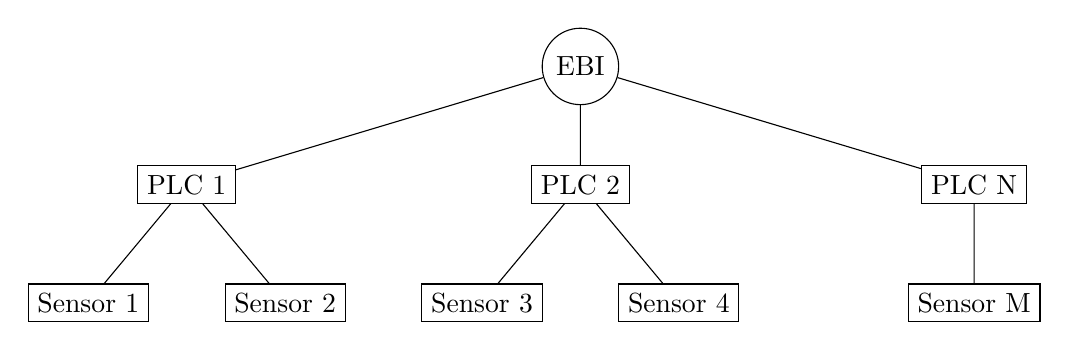
\begin{tikzpicture}[level 1/.style={sibling distance=5cm},
						level 2/.style={sibling distance=2.5cm}]
		\node[circle,draw]{EBI}
			child{
				node[rectangle,draw]{PLC 1}
					child[rectangle,draw]{node[rectangle,draw]{Sensor 1}}
					child[rectangle,draw]{node[rectangle,draw]{Sensor 2}}
				}
			child{
				node[rectangle,draw]{PLC 2}
					child{node[rectangle,draw]{Sensor 3}}
					child{node[rectangle,draw]{Sensor 4}}
				}
			child{
				node[rectangle,draw]{PLC N}
				child{node[rectangle,draw]{Sensor M}}
				}
		;
	\end{tikzpicture}
	\caption{Red industrial Gador.}
	\label{fig:redGador}
\end{figure}

\newpage

\section{Modelo de capas de la Internet de las Cosas}
\label{ch1IntroduccionTecnica}

% Presentación modelo de capas IoT
El proyecto realizado presentó una serie de desafíos a resolver, siendo el primero de ellos la variedad de tecnologías involucradas, tanto en la problemática a manipular como en la solución implementada.
Para introducir orden en la variedad de conocimientos que forman parte del sistema desarrollado, se introduce un modelo de capas de Internet de las cosas (IoT) \citep{dorsemaine2016new}.

% Enumeración de las capas y una breve descripción de cada una
El modelo de capas seleccionado separa los conocimientos en cinco categorías, las cuales son las capas de negocio, aplicación, procesamiento, red y percepción.
En la tabla \ref{tab:modeloCapas} se presenta un resumen de las funciones de cada capa.

\begin{table}[h]
	\centering
	\caption{\label{tab:modeloCapas}Modelo de capas IoT.}
	\begin{tabular}{c c}
		\toprule
		\textbf{Capa} & \textbf{Función}                         \\
		\midrule
		Negocio       & Establecer reglas y controlar el sistema \\
		Aplicación    & Interactuar con el usuario               \\
		Procesamiento & Almacenar y analizar los datos obtenidos \\
		Red           & Transportar los datos entre dispositivos \\
		Percepción    & Realizar mediciones o acciones en planta \\
		\bottomrule
		\hline
	\end{tabular}
\end{table}

% Capa de negocios
\subsection{Capa de negocios}
La capa de negocio suele tener una funcionalidad contable.
Esta capa puede ser la encargada de determinar y generar la facturación para cobrarle a los usuarios de la aplicación, como así también, resolver operaciones de transferencia de dinero.
La interacción en este nivel es con el personal que administra un sistema.
Se determina que permisos tiene cada usuario para manipular los servicios ofrecidos y se lleva adelante el registro de acciones y eventos relevantes para el normal funcionamiento del programa.
Un ejemplo de capa de negocio se puede observar en la figura \ref{fig:ch1EjemploNegocio}.

\begin{figure}[h]
	\centering
	\includegraphics[width=\textwidth]{./Figures/ch1EjemploNegocio.png}
	\caption{Software \emph{Checkmk}, ejemplo de capa de negocio. \citep{WEBSITE:checkmk}}
	\label{fig:ch1EjemploNegocio}
\end{figure}


% Capa de aplicación
\subsection{Capa de aplicación}
La experiencia que tiene el usuario al interactuar con la solución pertenece a la capa de aplicación.
Aquí se define como se presenta la interfaz gráfica que utilizan las personas, y es común utilizar un formato de sitio web.
Las páginas webs tienen la ventaja de ser indiferentes de la plataforma que utiliza el operador y solo importa que pueda ejecutar un navegador.

Actualmente, se construyen las interfaces siguiendo un modelo de diseño según el tipo de operación a realizar por el programa.
Si la solución abarca una interfaz hombre-máquina industrial que debe ser atendida durante toda una jornada laboral, se suele implementar una norma de manejo de situaciones anormales o ASM.
Si la aplicación es de uso intermitente, se puede usar un esquema de diseño material o \emph{Material Desing} que presenta una experiencia moderna y fluida, como se puede apreciar en la figura \ref{fig:ch1MaterialDesign}.

Para llevar adelante la interfaz seleccionada se utiliza un servidor que tiene como objetivo proveer los componentes gráficos al dispositivo utilizado.
Una manera de realizarlo es entregando al cliente una \emph{Single Web Application (SWP)}.
De esta manera se logra que el servidor otorgue todo el código necesario para que el dispositivo del usuario genere por sí mismo los componentes gráficos a mostrar.
Es importante que el código entregado pueda ser visualizado en múltiples tamaños de pantallas, ya que en la actualidad las personas utilizan ordenadores, tabletas y teléfonos móviles que presentan grandes diferencias en sus dimensiones.
Cuando una aplicación cumple con este requerimiento se la define como \emph{responsiva}.

% poner referencia de la figura en pie de página
% https://material.io/blog/mda-2020-winners
\begin{figure}[h]
	\centering
	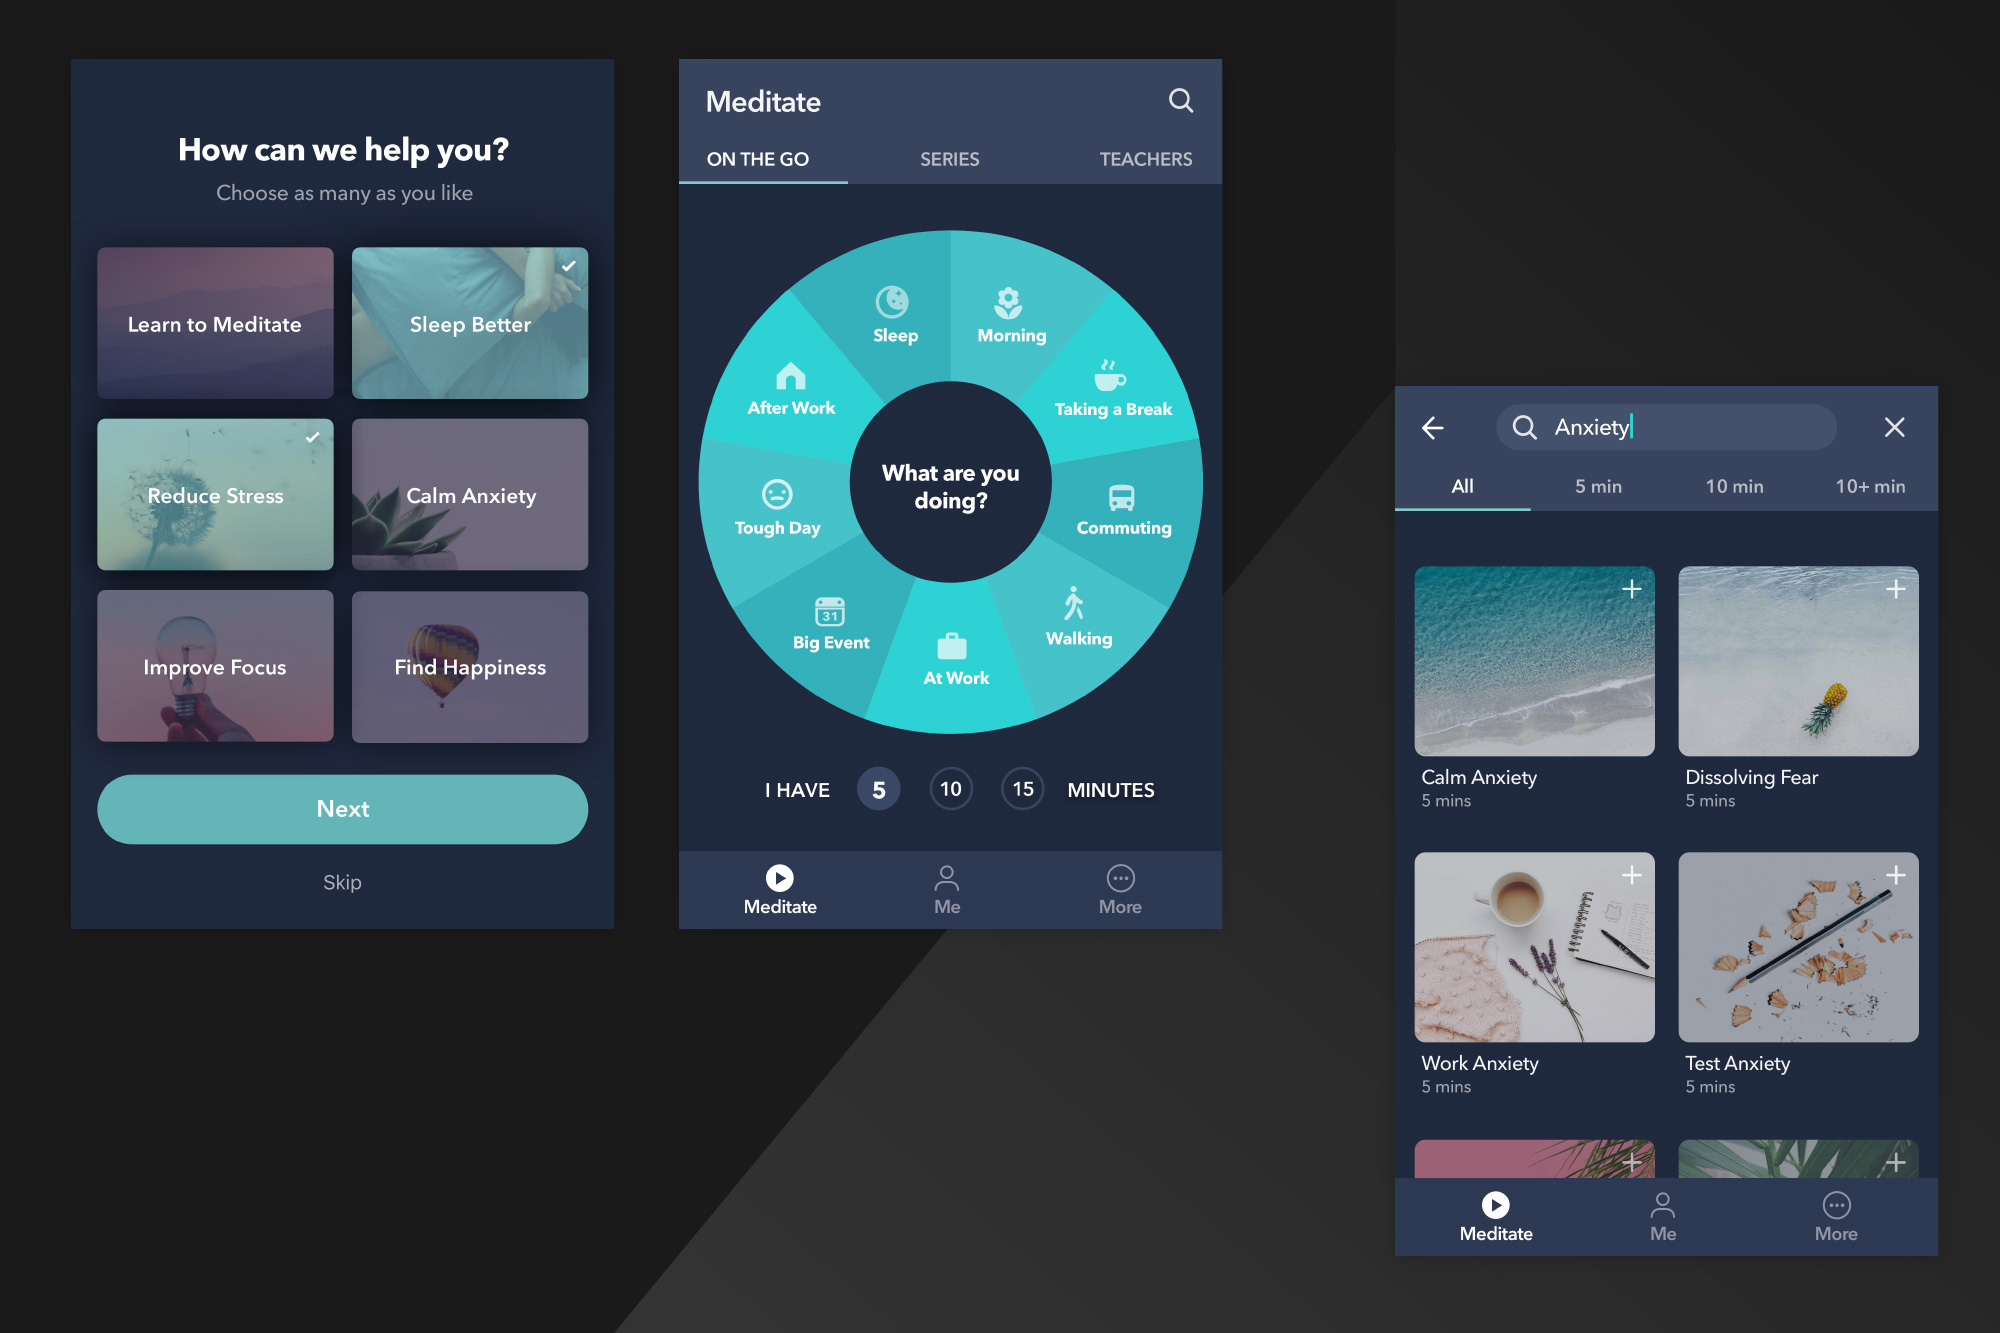
\includegraphics[width=\textwidth]{./Figures/ch1MaterialDesign.jpg}
	\caption{Ejemplo de interfaz de diseño material \citep{WEBSITE:Material}}.
	\label{fig:ch1MaterialDesign}
\end{figure}

\newpage

% Capa de procesamiento
\subsection{Capa de procesamiento}
Para alimentar de datos a la interfaz gráfica se necesita de la capa de procesamiento, que entrega el contenido a mostrar en pantalla. La información puede ser almacenada con distintas tecnologías.
Una de las principales es la tecnología de las bases de datos relacionales.
Este tipo de base de datos se basa en un esquema de tablas que se relacionan entre sí.
Estas tecnologías se las suelen llamar SQL y son utilizadas principalmente en datos de inventarios y sistemas de transacciones de dinero \citep{munar2014big}.
Existe otro grupo de bases de datos que se denominan no relacionales o NoSQL.
Esta categoría contiene a los siguientes tipos de bases de datos:

\begin{itemize}
	\item Clave-valor
	\item Orientada a documentos
	\item Orientada a columnas
	\item Orientada a grafos
\end{itemize}

% clave-valor
Las bases de datos clave-valor tratan los datos como una única colección que puede tener campos completamente distintos en cada registro \citep{nguyen2015zing}.
No existe entonces, ningún tipo de relación entre los miembros de la colección. El uso principal de esta tecnología es gestionar diccionarios dentro de la memoria volátil, ya que se pueden definir tiempos de vida para los datos. La muerte programada de un dato puede ser utilizada para gestionar las sesiones de usuario dentro del programa.

% documental
Almacenar los datos de manera documental significa que se agrupa la información siguiendo un criterio de entidades similares, lo cual no significa que exista una estructura rígida, sino que los datos tienen una naturaleza similar \citep{gutierrez2019herramienta}.
La persistencia se logra siguiendo formatos de codificación estándar, los cuales son:
% como \emph{XML}, \emph{YAML} y \emph{JSON}.

\begin{itemize}
	\item \emph{XML}
	\item \emph{YAML}
	\item \emph{JSON}
	\item \emph{BSON}
\end{itemize}

% columnas
Las bases de datos orientadas a columnas están pensadas para minimizar el tiempo de búsqueda, principalmente en series temporales.
La organización particular de este tipo de tecnologías es afín a los sistemas de IoT ya que los dispositivos de mediciones suelen generar un gran volumen de datos, que se pueden organizar como series temporales \citep{abadi2009column}.

% grafos
Una base de datos orientada a grafos presenta la información como nodos que se encuentran relacionados.
La diferencia fundamental con los sistemas relacionales es que los nodos no están organizados en tablas.
Además las relaciones que unen los nodos tienen atributos y no poseen una estructura definida.
Este tipo de tecnología permite utilizar la teoría de grafos y posibilita realizar consultas siguiendo modelos matemáticos que forman parte de esa rama de la ciencia \citep{gyssens1994graph}.
%Un ejemplo de esta tecnología se puede ver en la figura \ref{fig:ch1Grafo}.

%\begin{figure}[h]
%	\centering
%	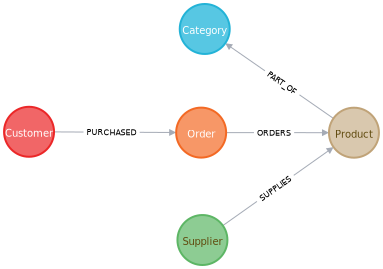
\includegraphics[width=.6\textwidth]{./Figures/ch1Grafo.png}
%	\caption{Ejemplo de base de datos orientada a grafos. \citep{WEBSITE:neo4j}}
%	\label{fig:ch1Grafo}
%\end{figure}

\newpage

% Capa de red
\subsection{Capa de red}
Se dispone de un repertorio de protocolos pertenecientes a la capa de red para lograr que los dispositivos se comuniquen entre sí.
Entre los mencionados a lo largo de esta memoria se encuentran Modbus, MQTT, HTTP y WebSocket. El manejo de estas tecnologías fue fundamental para lograr que las distintas partes del trabajo interactúen con el exterior.

% Modbus
Modbus es un protocolo que se diseñó para aplicaciones industriales.
Su prioridad es transmitir los datos manteniendo su integridad aún en ambientes donde el ruido eléctrico es elevado. El protocolo es público y gratuito, lo que provocó que se impusiera en un gran segmento del mercado ya que además es fácil de implementar.
Los dispositivos de una red Modbus tienen una dirección única y por lo general se asigna un equipo como maestro y el resto como esclavos. La arquitectura descripta presenta varias ventajas, pero no es adecuado para aplicaciones IoT.

% MQTT
Para interconectar a los dispositivos bajo un esquema de publicación-subscripción se utiliza el protocolo MQTT.
El protocolo está diseñado para conexiones en lugares remotos donde los dispositivos funcionan con un ancho de banda limitado.
El resultado es que los mensajes son pequeños y consumen poca batería de los equipos involucrados, por lo que se usa frecuentemente en los sistemas de IoT.
El tráfico es gestionado por un servidor del tipo broker que decide quienes son los destinatarios de un mensaje en particular, el resto de los dispositivos son clientes del broker.
Si un cliente desea transmitir datos, lo hace realizando una publicación a un determinado \emph{topic} y el broker se encarga de determinar quienes deben recibir la información enviada.
Quienes quieran obtener los datos publicados a un \emph{topic} en particular, se deben suscribir a él ante el broker.
Este al recibir una publicación de un cliente la transmite solo a los clientes que se encuentres subscritos, como se puede ver en el ejemplo de la figura \ref{fig:ch1MqttEjemplo}, donde el cliente 2 no obtiene los datos del sensor porque no se encuentra subscrito.

\begin{figure}[h]
	\centering
	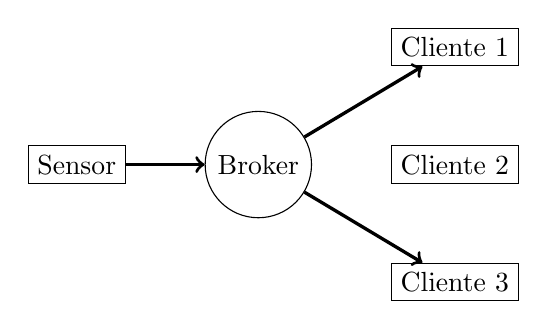
\begin{tikzpicture}
		\tikzstyle{broker} = [circle,draw=black]
		\tikzstyle{publish} = [rectangle,draw=black]
		\tikzstyle{subscribe} = [rectangle,draw=black]
		\tikzstyle{flecha} = [->,very thick]

		\node[publish] (p) {Sensor};
		\node[broker,right=of p] (b) {Broker};
		\node[subscribe, right=of b] (s2)	{Cliente 2};
		\node[subscribe,above=of s2] (s1) {Cliente 1};
		\node[subscribe, below=of s2] (s3) {Cliente 3};

		\draw[flecha] (p) edge (b);
		\draw[flecha] (b) edge (s1);
		\draw[flecha] (b) edge (s3);			
	\end{tikzpicture}
	\caption{Ejemplo de comunicación MQTT.}
	\label{fig:ch1MqttEjemplo}
\end{figure}

% HTTP y Websocket
El protocolo de transferencia de hipertexto (HTTP) está orientado a transacciones y sigue el esquema petición-respuesta entre un cliente y un servidor.
El cliente inicia la comunicación enviando una petición al servidor, este último entrega una respuesta y se cierra el canal.
Existe una variante del protocolo llamada HTTPS que agrega una capa de cifrado para que las comunicaciones sean seguras.

WebSocket es un protocolo similar a HTTP pero con la diferencia que la conexión es bidireccional.
Esto quiere decir que cuando se logra la conectar al cliente con el servidor, ambos pueden enviar información espontáneamente. Esta cualidad permite realizar transferencias de datos en vivo, con lo que se pueden lograr servicios de \emph{streaming} o \emph{chats}.

% Capa de percepción
\subsection{Capa de percepción}
Los sensores utilizados en una solución de IoT están incluidos en la capa de percepción.
Para que puedan formar parte del sistema se necesita que sean capaces de soportar alguno de los protocolos de comunicaciones mencionados. Dado que el desarrollo de estos dispositivos no formaron parte del proyecto realizado, no se ampliará en este tema.

% Despliegue de una solución
\subsection{Despliegue de una solución}
Teniendo definidos los componentes de las capas, se necesita lograr que todas las partes funcionen como una única entidad. Para lograr este objetivo existen tecnologías de despliegue y orquestación, que cumplen la función de interconectar y mantener los servicios para que trabajen en equipo. Tradicionalmente se solían utilizar máquinas virtuales pero actualmente ese enfoque está quedando en desuso en favor de las tecnologías de contenedores. Una máquina virtual acapara parte de una computadora y funciona como un ordenador independiente, mientras que un contenedor funciona como un sistema operativo independiente pero no acapara los recursos de la computadora principal.


\section{Estado del arte}
\label{ch1EstadoDelArte}

% La nube
En la sección \ref{ch1IntroduccionTecnica} se presentó un modelo de capas para analizar las tecnologías.
En esta sección se utiliza el mismo esquema para presentar las técnicas que conforman el estado del arte.

Es importante mencionar el concepto de nube, ya que las soluciones modernas se basan en utilizar este tipo de plataforma.
La nube se refiere a utilizar servicios y servidores provistos por un tercero.
Entre los sistemas más representativos se encuentran \emph{Amazon Web Service (AWS)}, \emph{Google Cloud} y \emph{Azure}.
Estas empresas ofrecen su infraestructura y una serie de facilidades que promueven un rápido desarrollo y despliegue en el mercado.

% Percepción
Los sensores o actuadores que utilizan corren un firmware específico.
Por ejemplo, si se decidió utilizar AWS lo más probable es que la capa de percepción ejecute \emph{AWS IoT Core} en sus dispositivos.
Este esquema es ampliamente utilizado a nivel \emph{enterprise}.
Por ejemplo, los laboratorios Bayer utilizan el ecosistema de AWS \citep{WEBSITE:AWSBayer}.

% Transporte
En la capa de transporte, los dispositivos se comunican usualmente utilizando los protocolos \emph{LoRaWAN}, \emph{Sigfox}, \emph{ZigBee} o \emph{Bluetooth}.
La selección del protocolo depende de las distancias a cubrir y de las necesidades energéticas.
Los sensores convergen luego a un punto de agregación.
Desde los puntos de agregación se suele transmitir los datos al servidor en la nube utilizando el protocolo MQTT.

% Procesamiento
En la capa de procesamiento se utiliza un esquema de datos de alta disponibilidad.
Esto se logra creando réplicas de los datos en distintos servidores.
Una de las réplicas se configura como maestro y el resto como esclavos.
El servidor maestro es quien se comunica con el exterior de la réplica y retransmite los nuevos datos a los esclavos.
Si un servidor maestro sufre un problema, uno de los esclavos se convierte en el nuevo maestro y se mantiene a la réplica funcionando sin interrupciones.

Los datos pueden ser divididos en \emph{shards}.
Esto se hace para dividir la base de datos según la aplicación.
Un ejemplo es separar los datos por región geográfica.
De esta manera los clientes de una región en particular pueden tener los servidores con los datos que suelen utilizar cerca de ellos.
Para que los \emph{shards} funcionen como una única base de datos, se dispone de un servidor \emph{router} que es la interfaz con el exterior.
El \emph{router} recibe las consultas o ingresos de nuevos datos y se encarga de utilizar el \emph{shard} correspondiente.
La configuración de este sistema se maneja desde un grupo de servidores destinados para tal fin, que suelen conformar una réplica donde solo se almacenan los datos de configuración.
Esta arquitectura de alta disponibilidad se conoce como granja de datos, se puede construir con mongoDB \citep{WEBSITE:mongodbSharding} y se encuentra representada en la figura \ref{fig:ch1DatosAltaDisponibilidad}.

\begin{figure}[h]
	\centering
	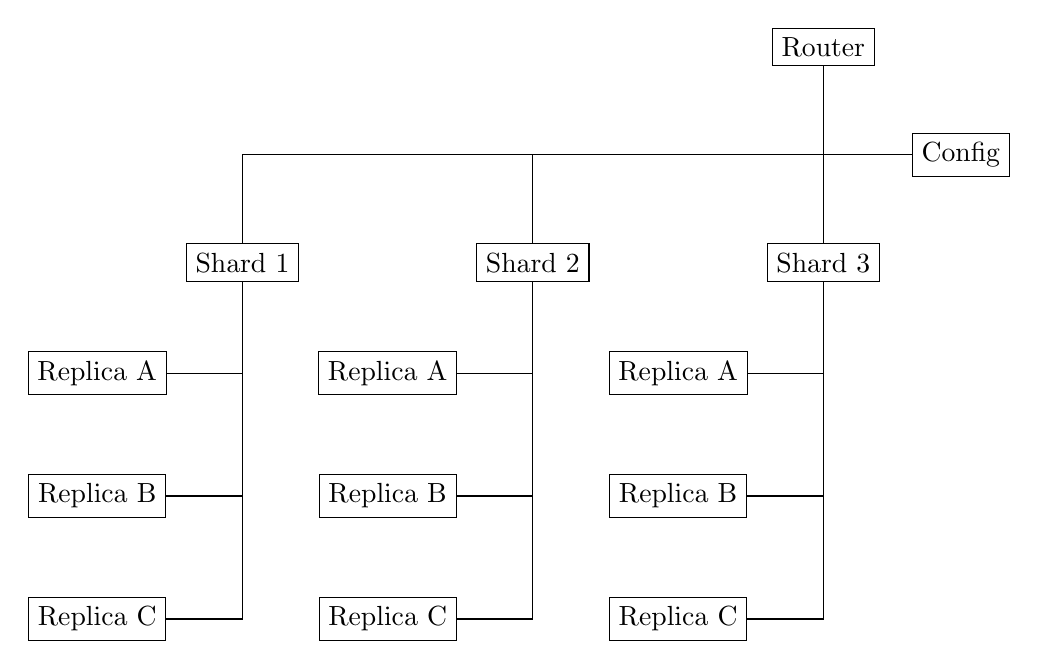
\begin{tikzpicture}		
		\tikzstyle{block} = [rectangle,draw=black]
				
		\node[block] (r) {Router};
		
		\node[below=of r] (aux) {};
		\node[block,right=of aux] (c) {Config};
		
		\node[block,below=of aux] (s3) {Shard 3};
		\node[left=of s3] (aux1) {};
		\node[block,left=of aux1] (s2) {Shard 2};
		\node[left=of s2] (aux2) {};
		\node[block,left=of aux2] (s1) {Shard 1};
		\node[left=of s1] (aux3) {};
		
		\node[block,below=of aux3] (ra1) {Replica A};
		\node[block,below=of ra1] (ra2) {Replica B};
		\node[block,below=of ra2] (ra3) {Replica C};
		
		\node[block,below=of aux2] (rb1) {Replica A};
		\node[block,below=of rb1] (rb2) {Replica B};
		\node[block,below=of rb2] (rb3) {Replica C};
		
		\node[block,below=of aux1] (rc1) {Replica A};
		\node[block,below=of rc1] (rc2) {Replica B};
		\node[block,below=of rc2] (rc3) {Replica C};
				
		\draw (r)--(s3);
		\draw (s1)|-(c);
		\draw (s2)|-(c);
		\draw (s3)|-(aux);
		\draw (c)--(aux);
		
		\draw (ra1)-|(s1);
		\draw (ra2)-|(s1);
		\draw (ra3)-|(s1);	
		
		\draw (rb1)-|(s2);
		\draw (rb2)-|(s2);
		\draw (rb3)-|(s2);
		
		\draw (rc1)-|(s3);
		\draw (rc2)-|(s3);
		\draw (rc3)-|(s3);
	\end{tikzpicture}
	\caption{Arquitectura de datos de alta disponibilidad.}
	\label{fig:ch1DatosAltaDisponibilidad}
\end{figure}

% Aplicación
La capa de aplicación se suele diseñar rápidamente con un framework dedicado a la construcción de interfaces gráficas.
Uno de los más utilizados es Angular, desarrollado por la empresa Google \citep{WEBSITE:Angulario}.
El estilo gráfico de diseño material presentado en la sección \ref{ch1IntroduccionTecnica} es la más utilizada.
Las plataformas de nube ofrecen sus propios sistemas para diseñar la aplicación sin necesidad de escribir demasiado código, pero estas facilidades generan erogaciones adicionales.

% Negocio
La plataforma de nube presenta una capa de negocios donde se puede controlar el tráfico del sistema en ejecución.
Desde allí se puede ver la facturación estimada o el consumo de crédito para mantener en funcionamiento el proyecto.
En esta capa se pueden cambiar las variables de entorno del sistema y se pueden controlar el estado de los componentes.
Es posible montar servicios que corran programas como \emph{Checkmk} o \emph{Grafana} para visualizar el estado de los dispositivos en campo \citep{betke2017real}. O se puede optar por usar los servicios que ofrezca la empresa de nube.

% Orquestación y despliegue
La tecnología que se suele utilizar para orquestar toda la solución es Kubernetes \citep{burns2018kubernetes}, ya que además de automatizar el despliegue, también permite ajustar la escala.
Ajustar la escala se refiere a la capacidad de crear una réplica de un servicio cuando uno de ellos está trabajando cerca de su límite de procesamiento.
Es un sistema basado en contenedores y crea un \emph{clúster} a partir de una plantilla donde se definen las reglas de escalamiento.

\section{Objetivos y alcance}
\label{objetivos}

% Objetivos
El objetivo principal que cumplió este trabajo fue demostrarle al cliente el potencial de las nuevas tecnologías y la posibilidad de integrarlas a sus actuales sistemas.
Se propuso crear una prueba de concepto para evaluar la viabilidad de futuros proyectos.
La creación de un sistema que pueda unir equipos que utilizan Modbus con aquellos que usan MQTT, es de relevancia en general para la industria local.

Otro objetivo importante fue el de utilizar las técnicas adquiridas durante la cursada de la especialización, con la finalidad de asentar los conocimientos a través de la práctica.

% Alcance
El trabajo se limitó a desarrollar el software a desplegar en un servidor.
Esto significa que no se contempló el desarrollo del hardware, en particular los sensores y los puntos de agregación.
El esquema del servidor en la red de Gador puede ser visualizado en la figura \ref{fig:esquemaProyecto}, donde el servidor denominado Nodos corresponde a la solución desarrollada.
El servidor puede comunicarse con EBI de la misma manera que lo logra un PLC.
Además tiene la capacidad de utilizar el protocolo MQTT para conectarse directamente con los sensores o a través de puntos de agregación.


\begin{figure}[h]
	\centering
	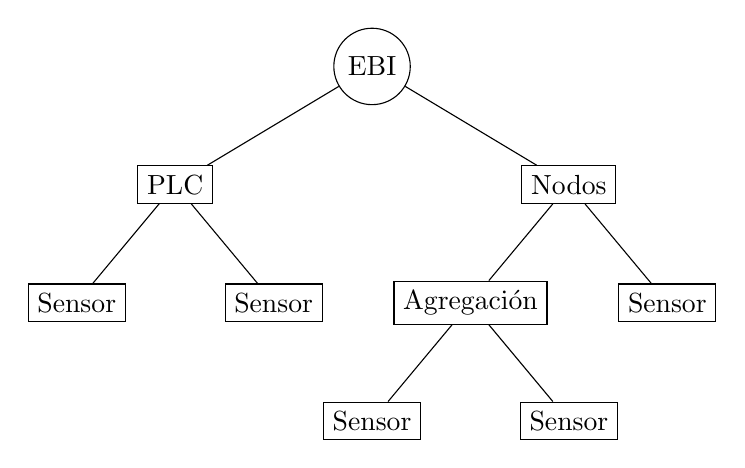
\begin{tikzpicture}[level 1/.style={sibling distance=5cm},
						level 2/.style={sibling distance=2.5cm}]
		\node[circle,draw]{EBI}
			child{
				node[rectangle,draw]{PLC}
					child[rectangle,draw]{node[rectangle,draw]{Sensor}}
					child[rectangle,draw]{node[rectangle,draw]{Sensor}}
				}
			child{
				node[rectangle,draw]{Nodos}
					child{
						node[rectangle,draw]{Agregación}
							child[rectangle,draw]{node[rectangle,draw]{Sensor}}
							child[rectangle,draw]{node[rectangle,draw]{Sensor}}
					}
					child{node[rectangle,draw]{Sensor}}
				}
		;
	\end{tikzpicture}
	\caption{Red industrial Gador.}
	\label{fig:esquemaProyecto}
\end{figure}

% Requerimientos
Una vez definidos los objetivos y el alcance del proyecto, se inició un proceso de negociación con el cliente.
Se buscó determinar cuales eran sus necesidades y sus temores respecto del proyecto.
Las conversaciones con el cliente dieron como resultado la siguiente lista de requerimientos:

\newpage

\begin{itemize}
	\item Debe integrarse a la infraestructura de Gador S.A. sin generar conflictos en otros sistemas.
	\item Debe crear tramas en el formato \emph{Enterprise Buildings Integrator} y enviarlas al servidor.
	\item Debe interpretar eventuales mensajes del servidor \emph{Honeywell}.
	\item Debe interpretar los mensajes de los sensores.
	\item Debe poder cambiar la frecuencia de lectura de mediciones.
	\item Debe poseer la capacidad de gestionar los ingresos de usuarios de forma segura.
	\item Debe permitir que por lo menos cinco usuarios accedan al sistema simultáneamente.
	\item Debe presentar una interfaz donde se monitoree el estado de los sensores
	\item Debe permitir elegir un sensor en particular para editarlo.
	\item Debe poseer un módulo de gestión de usuarios.
	\item Debe ser compatible con ordenadores de escritorio y smartphones.
	\item Las contraseñas no persistirán como texto plano.
	\item Debe persistir todas las modificaciones realizadas a la configuración de los sensores.
	\item Debe persistir las mediciones obtenidas.
\end{itemize}
\chapter{Introducción específica} % Main chapter title

\label{Chapter2}

%----------------------------------------------------------------------------------------
%	SECTION 1
%----------------------------------------------------------------------------------------
Este capítulo trata sobre los recursos tecnológicos de terceros que fueron utilizados en la producción del trabajo.

% Descripción de las plataformas tecnológicas que sostienen al trabajo
\section{Tecnologías utilizadas}

% docker
Para crear una arquitectura de microservicios se utilizó Docker, que es un software que permite el uso y creación de contenedores de Linux.
Un contenedor es una unidad que empaqueta el código de un programa junto con sus dependencias para aislar su funcionamiento.
Para crear un contenedor, el motor de Docker se vale de el concepto de imagen.
Las imágenes son entidades inmutables que cumplen la función de ser plantillas para crear contenedores.
Se puede visualizar a las imágenes como capturas del estado de un contenedor y a partir de estas capturas se pueden instanciar nuevos contenedores.
Los contenedores son entonces, unas abstracciones de la capa de aplicación de los sistemas Linux, como se puede visualizar en la figura \ref{fig:ch2WhatContainer}.
Varios contenedores pueden correr en el mismo ordenador como procesos aislados en el espacio de usuario sin generar ningún tipo de interferencias entre si.
La principal diferencia con las máquinas virtuales, es que estas son una abstracción del hardware del ordenador, transformando una única computadora en varios servidores.
Los contenedores en cambio, utilizan el kernel del sistema operativo del ordenador físico, no se abstrae un kernel, solo el espacio de aplicación o de usuario.

% docker files
Docker puede ser utilizado para construir imágenes definidas por el usuario.
Para lograrlo se usa un Dokerfile, que es un documento de texto que contiene todos los comandos que un usuario utilizaría para ensamblar una imagen.
El programador puede correr automáticamente una serie de comandos en sucesión al ejecutar una única orden sobre el Dockerfile.
Otra capacidad adicional es subir la imagen a un repositorio para ser descargado directamente sobre el entorno de producción.
De esta manera se facilita el despliegue de la aplicación, faltaría solamente, orquestar los contenedores para que trabajen en conjunto. 

% docker compose
La orquestación necesaria para la etapa de despliegue se logra utilizando Docker Compose.
Que según se indica en su documentación \citep{WEBSITE:WhatDockerCompose}, es una herramienta para definir y correr aplicaciones de Docker de múltiples contenedores.
Permite utilizar un archivo \emph{YAML} para configurar los servicios de la aplicación.
Con esta tecnología se pueden crear y comenzar todos los servicios de la configuración utilizando un único comando y finalmente se logra tener orquestada la solución.

\begin{figure}[h]
	\centering
	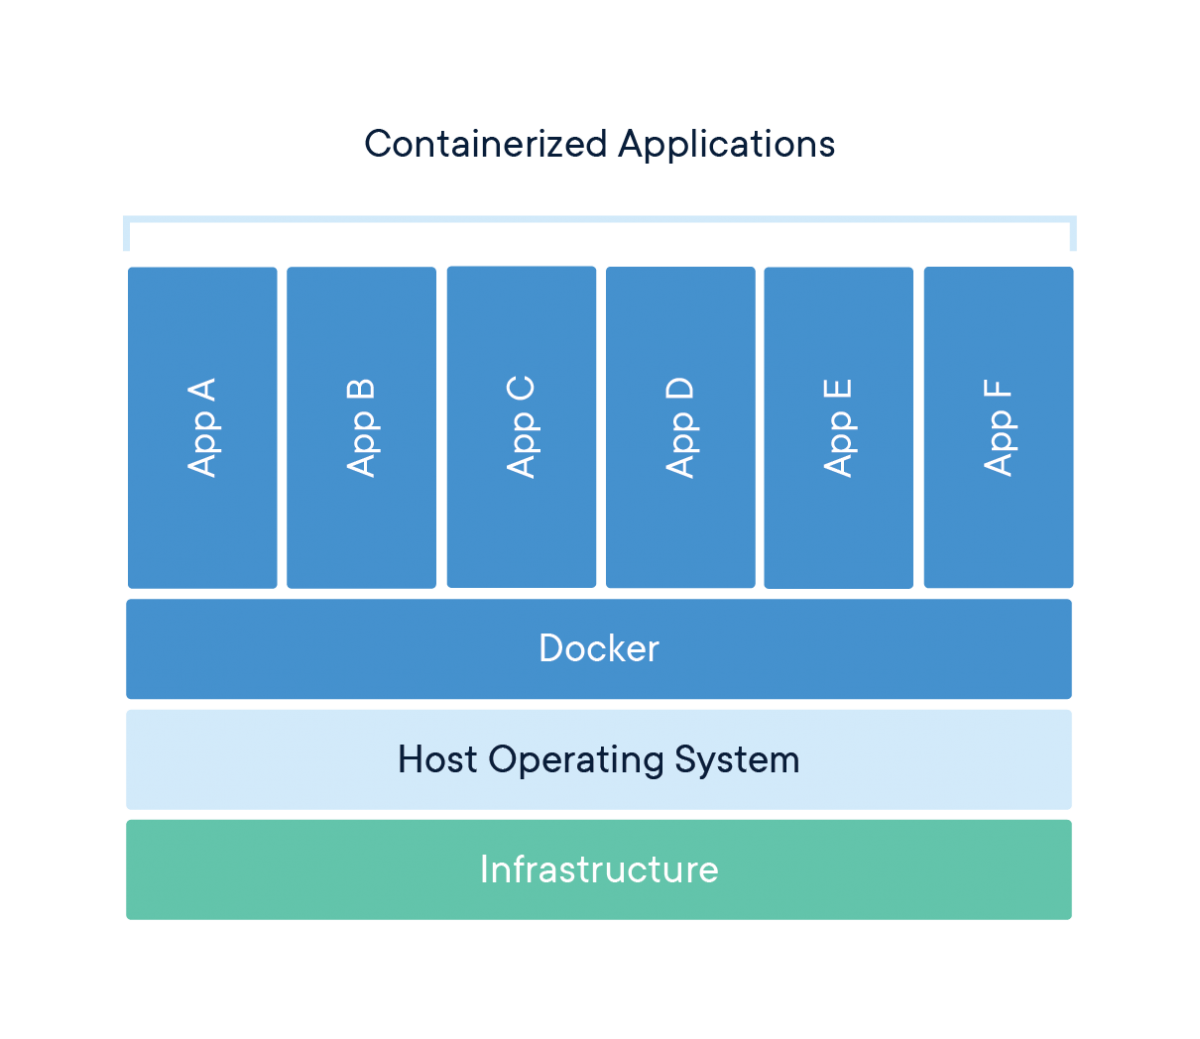
\includegraphics[width=\textwidth]{./Figures/ch2DockerContainer.png}
	\caption{Arquitectura de Docker. \citep{WEBSITE:WhatContainer}}
	\label{fig:ch2WhatContainer}
\end{figure}

% nodejs
El trabajo utiliza tecnologías web y la plataforma utilizada para implementarlas fue Nodejs, que es un servidor asincrónico y orientado a eventos que ejecuta JavaScript.
La orientación a eventos se consideró como una ventaja frente a las aplicaciones de concurrencia de múltiples hilos en el sistema operativo.
Principalmente porque no se utilizan candados y no existe la posibilidad de bloquear el servidor.
Una particularidad adicional es que fue diseñado para construir aplicaciones de red escalables y provee un gestor de paquetes muy fácil de utilizar.
Por estas razones y porque además fue una plataforma estudiada en la especialización, es que se la eligió para formar parte del trabajo.

% python
No todos los servicios del trabajo se realizaron con tecnologías relacionadas a JavaScript.
Particularmente se utilizaron una serie de bibliotecas y herramientas basadas en Python, que es un lenguaje de programación del tipo interpretado.
Este lenguaje posee una gran cantidad de recursos hechos por terceros y que se encuentran a disposición con licencias libres.
Si bien el lenguaje no fue visto con profundidad en la cursada, fue suficiente para entender su potencial.
Específicamente porque muchas de sus bibliotecas fueron útiles para desarrollar algunos de los servicios más pequeños del trabajo.
Es una tecnología que resultó muy útil y fue utilizada para acelerar la creación de las partes más livianas del sistema.
Partes que no justificaron el uso de una plataforma como Nodejs.

% mosquitto
Para implementar el protocolo MQTT se decidió utilizar paquetes y bibliotecas desarrollados por terceros.
La primera herramienta fue Eclipse Mosquitto que es un broker del protocolo.
Es liviano, no demanda grandes recursos y puede ser ejecutado en ordenadores monoplaca.
Es flexible ya que permite ser configurado de distintas maneras según las necesidades de la aplicación.
Existen varios niveles de calidad de servicio para seleccionar y también se pueden agregar usuarios de manera opcional.
Los usuarios poseen distintos permisos para publicar y suscribirse a diferentes \emph{topics}.
También es posible utilizar una capa de seguridad en los mensajes que se basa en la encriptación con llaves privadas y el uso de llaves públicas para realizar las lecturas.
Uno de los atractivos de la plataforma es la serie de programas utilitarios que incluye como recursos adicionales y que se integran en la terminal del sistema operativo.
Estas aplicaciones permiten realizar publicaciones y subscripciones para correr pruebas y además se pueden crear contraseñas encriptadas para los usuarios.

% mongodb
Para persistir la información durante la ejecución del trabajo se utilizó MongoDB.
"MongoDB es una base de datos distribuida, basada en documentos y de uso general diseñada para desarrolladores de aplicaciones modernas y para la era de la nube". \citep{WEBSITE:MongoHome}
Se decidió utilizar esta tecnología para la capa de procesamiento debido a la afinidad que posee para realizar aplicaciones IoT.
Además es la base de datos documental más utilizada actualmente \citep{WEBSITE:DBRanking} y se evaluó como aspecto relevante, ganar experiencia con esta tecnología.

% redis
Los contenedores que forman la aplicación deben compartir una memoria volátil para que el trabajo pueda funcionar correctamente.
Se eligió a Redis para que funcione como memoria compartida entre los componentes aislados dentro del trabajo.
Redis es un almacén de estructuras de datos en memoria y puede ser usado como una base de datos, una \emph{caché} de memoria y un broker para crear un bus de eventos.
Esta tecnología permite hacer persistencia de datos pero solo en el esquema de clave-valor y permite también establecer los tiempos de vida para los datos.
Los tiempos de vida de los datos se utilizaron en el trabajo para gestionar las sesiones de los usuarios.
Si una persona pasa demasiado tiempo sin interactuar con la aplicación tiene que volver a ingresar su usuario y contraseña para seguir utilizando el sistema con normalidad.	
	
% Descripción de las dependencias del trabajo
\section{Bibliotecas y paquetes de terceros}

% Angular & Angular Material
Para implementar la capa de aplicación se utilizó un framework de diseño de interfaces gráficas llamado Angular y se creó una SWA.
Se desarrolla el código usando el lenguaje TypeScript que es un \emph{superset} de JavaScript.
Está basado en el paradigma de componentes para generar aplicaciones escalables y poder reutilizar el código escrito en otros trabajos.
Pone a disposición una colección de bibliotecas para manejar formularios, comunicaciones cliente-servidor, \emph{routing}, entre otras funcionalidades.
Tiene entre sus facilidades ofrecidas, un cliente de terminal que acelera los tiempos de desarrollo.
Por todas estas ventajas, se decidió inclinarse por este framework.

El estilo empleado en el trabajo fue el de diseño material.
Para lograrlo se trabajó con Angular Material que es una biblioteca de componentes de interfaz gráfica para Angular.
Está pensada para construir una experiencia consistente y funcional, adhiriendo con los principios de diseño más utilizados.
Estos principios se refieren a la portabilidad entre navegadores y la independencia de dispositivos.

% express & cors
Se necesitó crear una \emph{REST API} y para lograrlo se usó un framework para realizar servidores con Nodejs denominado Express.
El framework está pensado para construir aplicaciones webs e interfaces de programación de aplicaciones (API).
Una API se encarga de definir las interacciones entre múltiples programas o puede intermediar entre componentes de hardware y software.
Express es la biblioteca más utilizada para trabajar con Nodejs. \citep{WEBSITE:Express}

Para solucionar el problema de intercambio de recursos de origen cruzado del frontend (CORS) se utilizó la biblioteca CORS para Nodejs.
CORS es una solución que permite acceder a recursos restringidos de un dominio diferente al del frontend.

% paho MQTT
Eclipse Paho es una biblioteca MQTT que está disponible para varios lenguajes de programación.
En el trabajo realizado se utilizó para darle conectividad a los servicios programados en Python.
La biblioteca provee una clase cliente que habilita la comunicación con un broker MQTT.
Se ofrece además, una serie de funciones auxiliares que permiten codificar el programa con mayor facilidad.

% mqttjs
Se necesitó un recurso que ofrezca de capacidades MQTT al código escrito en JavaScript y para esa misión se usó MQTTjs.
MQTTjs es una biblioteca que provee de las herramientas para crear un cliente MQTT en Nodejs y en un navegador.
Se lo puede instalar de forma global en el sistema operativo para hacer uso de las herramientas de terminal que ofrece.
Las herramientas permiten hacer pruebas de subscripción y publicación de mensajes.

% wsjs
Para cumplir con el requerimiento de la sección \ref{objetivos} que demanda ver en vivo las mediciones al calibrar un instrumento, se utilizó WS. 
Esta dependencia es una biblioteca de Nodejs que se usa para realizar servidores con la capacidad de entablar una conexión WebSocket.
Es fácil de utilizar y es altamente configurable.
Se decidió incorporarla al trabajo debido a que la documentación es completa y simple de entender.

% mongoose
Mongoose es una biblioteca de modelado de datos de objetos(ODM).
Un ODM gestiona las relaciones entre los datos, provee de una validación de esquema y se usa para traducir los objetos del programa en ejecución en una representación dentro de la base de datos.
La biblioteca se creó para trabajar con MongoDB y está disponible para la plataforma Nodejs.

% bcrypt jsonwebtoken
Se necesitó cumplir con las necesidades de seguridad que se enumeraron en la sección \ref{objetivos}, para lograrlo se usaron dos bibliotecas compatibles con Nodejs.
Bcrypt es una biblioteca que contiene funciones para encriptar contraseñas.
La encriptación se basa en un esquema de \emph{hashing} e incorpora una \emph{salt} para proteger los datos de un ataque \emph{rainbow table}.
Para darle resistencia a los ataques de búsqueda por fuerza bruta, la biblioteca implementa una función adaptativa que por cada iteración se vuelve más lenta.
Esto hace que su resistencia sea fuerte aún cuando el ordenador que realiza el ataque sea potente.
Por estas razones se decidió usar este recurso en el trabajo, con la idea de proteger las contraseñas de los usuarios evitando que persistan como texto plano.

% jsonwebtoken
La segunda bibliteca utilizada para cumplir con los requerimientos de seguridad fue Jsonwebtoken.
Que es un paquete que permite crear un \emph{JavaScript Web Token (JWT)}.
JWT es un estándar que se utiliza para la fabricación de \emph{tokens} de acceso que permiten identificar una entidad y determinar cuales son sus privilegios en el sistema.
El token está formado por una cabecera, una carga útil y una firma.
La cabecera identifica el algoritmo de encriptación y el tipo de token.
La carga útil lleva consigo la información relevante para el funcionamiento de la aplicación.
Finalmente la firma cierra el token para certificar la llave privada del servidor.
Es relevante mencionar que la biblioteca está diseñada para funcionar con Nodejs

% chai & mocha
La biblioteca Chai ofrece herramientas para hacer pruebas del software escrito.
Fue diseñada para Nodejs y puede ser integrada a cualquier framework de JavaScript.
En el trabajo fue combinado con Mocha, que es un framework de automatización de pruebas para Nodejs.
Las pruebas obtenidas al combinar estos dos recursos fueron fundamentales para detectar comportamientos no deseados.

% pyModbusTCP
Para que el código escrito en Python pueda utilizar el protocolo ModbusTCP se usó la biblioteca PyModbusTCP.
Este recurso permite crear un cliente para acceder a un servidor o bien crear una aplicación que se comporte como esclavo.

% oitc/modbus-server
Oitc/modbus-server es un servidor ModbusTCP realizado en Python y disponible como imagen de Docker.
Está configurado para utilizar el puerto 5020 para evitar problemas de permisos con el sistema operativo. \citep{WEBSITE:dockerhubModbus}
El sistema de orquestación corrige el puerto al conectar el 5020 del contenedor con el 502 del ordenador.

Todas las dependencias del trabajo se pueden visualizar en la tabla \ref{tab:dependencias}.

\begin{table}[h]
	\centering
	\caption{\label{tab:dependencias}Dependencias del trabajo.}
	\begin{tabular}{c c}
		\toprule
		\textbf{Dependencia}      & \textbf{Función}                          \\
		\midrule
		Docker             & Motor de contenedores                     \\
		Docker Compose     & Orquestación de contenedores              \\
		Dockerfile         & Creación de imágenes para Docker          \\
		Nodejs             & Servidor para JavaScript                  \\
		Python             & Lenguaje para los servicios ligeros       \\
		Eclipse Mosquitto  & Broker MQTT de la aplicación              \\
		MongoDB            & Base de datos                             \\
		Redis              & Memoria compartida entre contenedores     \\
		Angular            & Framework para crear la SWA               \\
		Angular Material   & Componentes gráficos para Angular         \\
		Express            & REST API para Nodejs                      \\
		CORS               & Intercambio de recursos de origen cruzado \\
		Paho MQTT          & Biblioteca MQTT para Python               \\
		MQTTjs             & Biblioteca MQTT para Nodejs               \\
		WS                 & Funcionalidad WebSocket para Nodejs       \\
		Mongoose           & ODM para Nodejs y MongoDB                 \\
		Bycrypt            & Seguridad de contraseñas                  \\
		JsonWebToken       & Seguridad de sesiones de usuarios         \\
		Chai               & Pruebas unitarias para JavaScript         \\
		Mocha              & Pruebas automáticas para Nodejs           \\
		PyModbusTCP        & Biblioteca Modbus para Python             \\
		Oitc/modbus-server & Servidor Modbus                           \\
		\bottomrule
		\hline
	\end{tabular}
\end{table}

% Descripción del sistema marca Honeywell que funciona en planta.
\newpage
\section{Sistema propietario del cliente}

Como se explicó en el capítulo \ref{Chapter1}, el trabajo se basa en lograr integrarse al sistema que Gador tiene en ejecución. Esta sección explica con mayor detalle la naturaleza de este producto.

EBI es un sistema de automatización de edificios y gestión empresarial creado por la firma Honeywell.
Ofrece herramientas para dotar a las dependencias de la empresa de la inteligencia necesaria para incrementar la comodidad, mejorar la seguridad y reducir los costos operativos.

La solución tiene la facultad de gestionar una red de edificios a través de una única interfaz gráfica. Pretende reducir los tiempos de respuesta frente a situaciones anormales y mejorar la seguridad.
Esta tecnología es compatible con dispositivos y software de terceros, con la idea de ofrecer escalabilidad.

Este software es un ecosistema de módulos que pueden ser adquirido a través de licencias para agregar las siguientes funcionalidades:

\begin{itemize}
	\item Gestión de consumo energético
	\item Seguridad de vida
	\item Control de acceso e intrusión
	\item Vídeo vigilancia
\end{itemize}

Las distintas licencias que vende Honeywell permiten que EBI utilice los protocolos BACNet, OPC, LonWorks y ModbusTCP.
Gador adquirió el producto con la licencia ModbusTCP para conectar sus PLCs de variadas marcas.
Como se puede observar en la figura \ref{fig:ch2EBI1}, se utiliza el software para visualizar los sensores de los distintos cuartos de producción y depósitos.
En la figura \ref{fig:ch2EBI2} se puede visualizar que EBI está a cargo del control ambiental de las plantas del cliente.
Este sistema es el corazón de la gestión de edificios de la compañía y determinó los requerimientos que propuso Gador.

La importancia de EBI para mantener la operación diaria de las plantas de Gador hizo que se limitara el acceso para hacer pruebas.
El servidor que corre este programa se encuentra custodiado con gran celo dentro de la compañía.
No se pudieron correr pruebas directamente sobre el ambiente de producción, solo se pudo utilizar por algunas horas una máquina virtual entregada con una licencia de evaluación que tuvo seis horas de duración.

\begin{figure}[h]
	\centering
	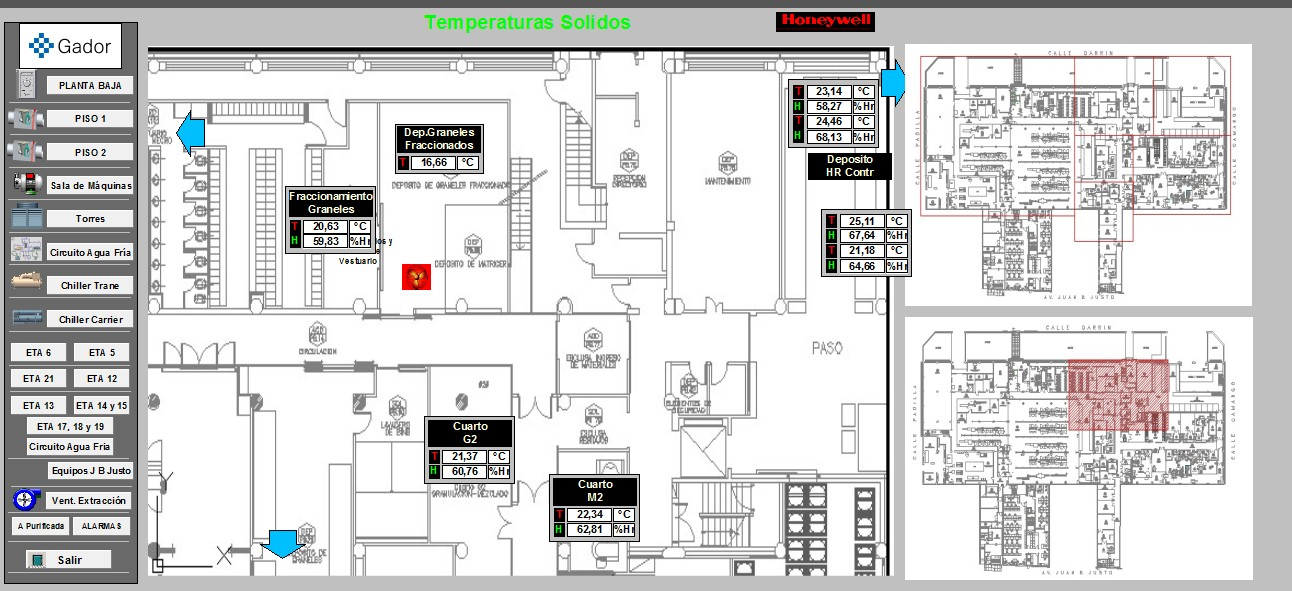
\includegraphics[width=\textwidth]{./Figures/ch2EBI1.jpg}
	\caption{Control de temperatura de sólidos.}
	\label{fig:ch2EBI1}
\end{figure}

\begin{figure}[h]
	\centering
	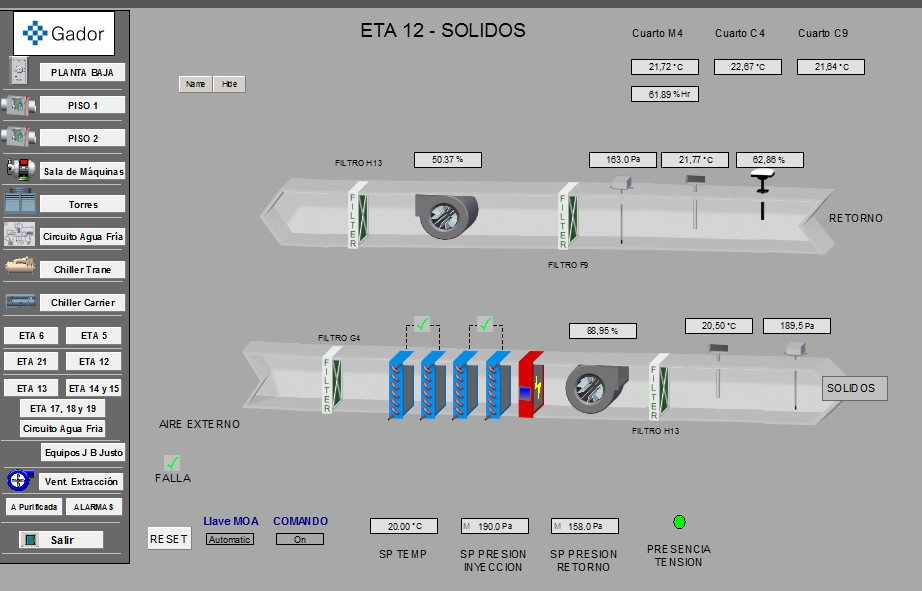
\includegraphics[width=\textwidth]{./Figures/ch2EBI2.jpg}
	\caption{Unidad de tratamiento de aire de sólidos.}
	\label{fig:ch2EBI2}
\end{figure} 
\chapter{Diseño e implementación} % Main chapter title

\label{Chapter3} % Change X to a consecutive number; for referencing this chapter elsewhere, use \ref{ChapterX}

\definecolor{mygreen}{rgb}{0,0.6,0}
\definecolor{mygray}{rgb}{0.5,0.5,0.5}
\definecolor{mymauve}{rgb}{0.58,0,0.82}

%%%%%%%%%%%%%%%%%%%%%%%%%%%%%%%%%%%%%%%%%%%%%%%%%%%%%%%%%%%%%%%%%%%%%%%%%%%%%
% parámetros para configurar el formato del código en los entornos lstlisting
%%%%%%%%%%%%%%%%%%%%%%%%%%%%%%%%%%%%%%%%%%%%%%%%%%%%%%%%%%%%%%%%%%%%%%%%%%%%%
\lstset{ %
  backgroundcolor=\color{white},   % choose the background color; you must add \usepackage{color} or \usepackage{xcolor}
  basicstyle=\footnotesize,        % the size of the fonts that are used for the code
  breakatwhitespace=false,         % sets if automatic breaks should only happen at whitespace
  breaklines=true,                 % sets automatic line breaking
  captionpos=b,                    % sets the caption-position to bottom
  commentstyle=\color{mygreen},    % comment style
  deletekeywords={...},            % if you want to delete keywords from the given language
  %escapeinside={\%*}{*)},          % if you want to add LaTeX within your code
  %extendedchars=true,              % lets you use non-ASCII characters; for 8-bits encodings only, does not work with UTF-8
  %frame=single,	                % adds a frame around the code
  keepspaces=true,                 % keeps spaces in text, useful for keeping indentation of code (possibly needs columns=flexible)
  keywordstyle=\color{blue},       % keyword style
  language=[ANSI]C,                % the language of the code
  %otherkeywords={*,...},           % if you want to add more keywords to the set
  numbers=left,                    % where to put the line-numbers; possible values are (none, left, right)
  numbersep=5pt,                   % how far the line-numbers are from the code
  numberstyle=\tiny\color{mygray}, % the style that is used for the line-numbers
  rulecolor=\color{black},         % if not set, the frame-color may be changed on line-breaks within not-black text (e.g. comments (green here))
  showspaces=false,                % show spaces everywhere adding particular underscores; it overrides 'showstringspaces'
  showstringspaces=false,          % underline spaces within strings only
  showtabs=false,                  % show tabs within strings adding particular underscores
  stepnumber=1,                    % the step between two line-numbers. If it's 1, each line will be numbered
  stringstyle=\color{mymauve},     % string literal style
  tabsize=2,	                   % sets default tabsize to 2 spaces
  title=\lstname,                  % show the filename of files included with \lstinputlisting; also try caption instead of title
  morecomment=[s]{/*}{*/}
}


%----------------------------------------------------------------------------------------
%	SECTION 1
%----------------------------------------------------------------------------------------
En este capítulo se detallan los componentes realizados por el autor de esta memoria.
Se explica como se crearon los servicios y como se interconectaron para lograr que todo funcione como una única solución.

\section{Arquitectura y orquestación}
Esta sección trata sobre la conexión entre los servicios del trabajo y su despliegue automático.

Para planificar la orquestación se analizaron los servicios que debían ser accesibles desde entidades externas al servidor.
En la figura \ref{fig:ch3EsquemaTrabajo} se pueden observar las conexiones lógicas entre los contenedores.
Destacadas en color rojo, se encuentran las entidades externas que interactúan con el servidor Nodos.
Las interconexiones se simplificaron al crear una capa de puente de red que corre sobre el \emph{Daemon} de Docker.
El resultado es que cada contenedor pasa a tener una dirección de ip dentro del entorno.
La creación de la red se logró con el código \ref{cod:dcNetwork}.

\begin{figure}[h]
	\centering
	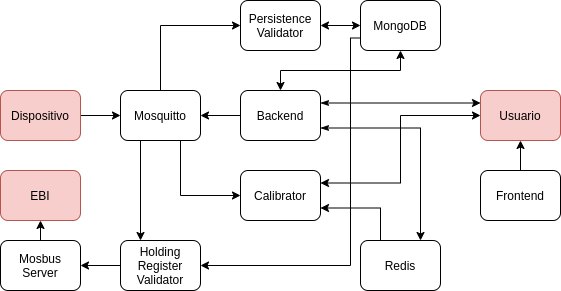
\includegraphics[width=\textwidth]{./Figures/ch3EsquemaTrabajo.png}
	\caption{Esquema de conexión de los servicios.}
	\label{fig:ch3EsquemaTrabajo}
\end{figure}

\begin{lstlisting}[label=cod:dcNetwork,caption=Red de interconexión Docker Compose.]
networks: 
	iot:
		driver: bridge
\end{lstlisting}

\subsection{Servidor Modbus}

El servicio modbus-server se comunica al exterior utilizando el puerto 502.
El puerto pertenece a la lista de protocolos bien conocidos o puertos de sistema.
Esta condición hace posible que existan problemas con los permisos que el usuario tiene dentro del sistema operativo.
Como se puede observar en el código \ref{cod:dcModbusServer}, se conectó el puerto 502 del ordenador con el 5020 dentro de la red de Docker.
En general, es una buena práctica que los puertos internos de la red no sean puertos de sistema para no generar conflictos de permisos y conectarlos a puertos de protocolos según sea necesario.
Para evitar usar direcciones ip en el código de los servicios se utilizó el parámetro hostname para utilizar el servicio de sistema de nombres de dominio (DNS) que corre dentro del \emph{Daemon} de Docker.

\begin{lstlisting}[label=cod:dcModbusServer,caption=Orquestación del servidor Modbus.]
modbus-server:
	image: oitc/modbus-server
	container_name: modbus-server
	hostname: modbus-server
	restart: always
	ports:
		- '502:5020'
	expose: 
    	- '5020'
	networks: 
		- iot
\end{lstlisting}

\subsection{Broker Mosquitto}

El servicio Mosquitto se configuró con tres volúmenes que conectan al contenedor con archivos no efímeros que persisten la información.
De esta manera se asegura que el contenedor muestre un comportamiento correcto.
Como se puede apreciar en el código \ref{cod:dcMosquitto}, se encuentran los archivos de configuración de usuarios y de lista de control de acceso (acl).
Con esta configuración se evita que dispositivos anónimos puedan utilizar el broker y que además solo se puedan utilizar los \emph{topics} designados.
Adicionalmente, los distintos usuarios tienen diferentes permisos según el \emph{topic}.
Así se logra una mayor confiabilidad y seguridad en el manejo de los mensajes.

\begin{lstlisting}[label=cod:dcMosquitto,caption=Orquestación del broker Mosquitto.]
mosquitto:
	image: eclipse-mosquitto
	container_name: mosquitto
	hostname: mosquitto
	restart: always
	volumes: 
		- ./mosquitto/mosquitto.conf:/mosquitto/config/mosquitto.conf
		- ./mosquitto/users.txt:/mosquitto/config/users.txt
		- ./mosquitto/acl.txt:/mosquitto/config/acl.txt
	expose: 
		- '1883'
		- '9001'
	ports: 
		- '1883:1883'
		- '9001:9001'
	networks: 
		- iot
\end{lstlisting}

\subsection{Validación de registros Modbus}

El servicio Holding Registers Validator (hrv) tiene la particularidad de depender de otros servicios, como se puede ver en el cógigo \ref{cod:dcHRV}.
El contenedor no puede ser creado hasta que los servicios listados como dependencias se encuentren activos.
Esto se hace de esta manera para evitar que el contenedor genere excepciones y se reinicie varias veces durante el despliegue se la solución.
Además no es posible saber si el comportamiento final del contenedor puede quedar indefinido.
Es importante mencionar que este servicio no tiene salida al exterior y no queda visible por la falta de campos \emph{ports}.

La imagen para construir el contenedor no existe y debe ser creada al momento del despliegue.
Para lograrlo se utiliza el campo \emph{build}, en donde se especifica la ruta al Dockerfile que contiene la receta.
La imagen queda guardada con el nombre vaca/hrv, de esta manera, no es necesario volver a construirla si se decide reiniciar la aplicación.

\begin{lstlisting}[label=cod:dcHRV,caption=Orquestación del servicio hrv.]
hrv:
	build: ./holdingRegistersValidator/
	image: vaca/hrv
	container_name: hrv
	hostname: hrv
	restart: always
	expose: 
		- '1883'
		- '5020'
	depends_on: 
		- 'mosquitto'
		- 'mongo'
		- 'modbus-server'
	networks: 
		- iot
\end{lstlisting}

El Dockerfile que fabrica la imagen puede verse en el código \ref{cod:dfHRV}.
Este código es común para todos los Dockerfiles que construyen imágenes para los servicios realizados en Python.
Se utiliza Alpine Linux como imagen base y se genera el usuario y grupo \emph{pythonuser}.
El usuario es quien corre el servicio dentro del contenedor y se definió un comando a ejecutar al momento de crearlo.
Quedan indicados en este archivo cuales son puertos que se pueden usar para la red puente.

\begin{lstlisting}[language=bash,label=cod:dfHRV,caption=Dockerfile del servicio hrv.]
FROM python:3.8-alpine
LABEL maintainer="Gonzalo Nahuel Vaca <vacagonzalo@gmail.com>"
RUN addgroup -g 1000 -S pythonuser && \
	adduser -u 1000 -S pythonuser -G pythonuser && \
	mkdir -p /app && \
	pip3 install pyModbusTCP && \
	pip3 install paho-mqtt && \
	pip3 install pymongo
ADD --chown=root:root app/* /app/
USER pythonuser
EXPOSE 1883 27017 5020/tcp
CMD [ "python", "-u", "/app/service.py" ]
\end{lstlisting}

\subsection{MongoDB}

El servicio MongoDB no tiene salida al exterior del servidor y su configuración se puede ver en el código \ref{cod:dcMongo}.
La configuración tiene la particularidad de introducir un comando a la hora de crear el contenedor.
Así se le indica al motor de MongoDB cual puerto debe escuchar.
Además se crea un volumen donde figuran una serie de archivos que pueblan la base de datos con información para construir una maqueta.
Esta maqueta fue utilizada para realizar la demostración al cliente.
Los archivos son devices.js, measurements.js, seed.js y users.js.
El archivo devices.js crea una serie de dispositivos ficticios.
El archivo measurements.js inserta una serie de mediciones que provienen de los dispositivos ficticios creados por devices.js.
El script users.js genera una serie de usuarios con distintos permisos, con el fin de probar la capacidad de autentificar las sesiones.
Finalmente seed.js es quién carga todos los datos en MongoDB.
Según se puede ver en el código \ref{cod:dcSeed}, las mediciones fueron cargadas múltiples veces para generar un volumen de datos que sirviera para realizar pruebas.

\begin{lstlisting}[label=cod:dcMongo,caption=Orquestación de MongoDB.]
mongo:
	image: mongo
	container_name: mongo
	hostname: mongo
	command: mongod --bind_ip_all --port 27017
	expose: 
		- '27017'
	volumes: 
		- ./mongodb/scripts:/scripts
	networks:
		- iot
\end{lstlisting}

\begin{lstlisting}[label=cod:dcSeed,caption=Seed de la base de datos.]
use gador;
load("scripts/devices.js")
load("scripts/users.js")
load("scripts/measurements.js")
load("scripts/measurements.js")
load("scripts/measurements.js")
load("scripts/measurements.js")
load("scripts/measurements.js")
load("scripts/measurements.js")
load("scripts/measurements.js")
load("scripts/measurements.js")
load("scripts/measurements.js")
\end{lstlisting}

\subsection{Validación de mediciones}

El servicio Persistence Validator (pv) está definido en el código \ref{cod:dcPV} y se puede observar que la imagen no existe.
Debe ser construida utilizando un Dockerfile.
Como el servicio fue realizado en Python, el Dockerfile necesario para construir la imagen es prácticamente idéntico al visto en el código \ref{cod:dfHRV}.

\newpage

\begin{lstlisting}[label=cod:dcPV,caption=Orquestación del servicio pv.]
	pv:
		build: ./persistenceValidator
		image: vaca/pv
		container_name: pv
		hostname: pv
		restart: always
	expose: 
		- '1883'
		- '27017'
	depends_on: 
		- 'mosquitto'
		- 'mongo'
	networks: 
		- iot
\end{lstlisting}

\subsection{Backend}

Para orquestar el servicio backend, según el código \ref{cod:dcBackend}, se utilizó el puerto 8080 del ordenador para permitir la comunicación con una entidad externa.
La imagen para crear el contenedor debe ser construida y para tal fin se usó el Dockerfile que se puede observar en el código \ref{cod:dfBackend}.
El Dockerfile parte de la imagen oficial de Nodejs y copia los archivos de dependencias dentro del contenedor auxiliar.
Con este contenedor se descargan las bibliotecas necesarias.
Luego se copia el código fuente de la aplicación y finalmente se configura la inicialización del servidor Nodejs como comando por defecto.

\begin{lstlisting}[label=cod:dcBackend,caption=Orquestación del servicio Backend.]
backend:
	build: ./backend
	image: vaca/backend
	container_name: backend
	hostname: backend
	expose: 
		- '1883'
		- '6379'
		- '27017'
	ports: 
		- '8080:8080'
	depends_on:
		- 'mosquitto' 
		- 'mongo'
		- 'redis'
	networks: 
		- iot
\end{lstlisting}

\begin{lstlisting}[language=bash,label=cod:dfBackend,caption=Dockerfile del servicio Backend.]
FROM node
LABEL maintainer="Gonzalo Nahuel Vaca <vacagonzalo@gmail.com>"
WORKDIR /usr/src/app
COPY package*.json ./
RUN npm install
COPY . .
EXPOSE 1883 6379 8080 27017
CMD ["node", "./src/app.js"]
\end{lstlisting}

\subsection{Servicio de calibración}

El servicio Calibrator es una aplicación de Nodejs y fue orquestada de manera similar al servicio Backend.
Su configuración se puede observar en el código \ref{cod:dcCalibrator}.
El Dockerfile necesario para crear su imagen es prácticamente idéntico al mostrado en el código \ref{cod:dfBackend}.

\begin{lstlisting}[label=cod:dcCalibrator,caption=Orquestación del servicio Calibrator.]
calibrator:
	build: ./calibrator
	image: vaca/calibrator
	container_name: calibrator
	hostname: calibrator
	expose: 
		- '1883'
		- '9999'
	ports:
		- '9999:9999'
	depends_on: 
		- 'mosquitto'
	networks: 
		- iot
\end{lstlisting}

\subsection{Redis}

El servicio Redis fue creado a partir de la imagen oficial de Redis que se encuentra disponible en Dockerhub. \citep{contrib:redis}
Como no tiene exposición al exterior del servidor, no se necesitó realizar ninguna configuración adicional.
Es importante aclarar que si bien se puede aplicar una capa de seguridad, no es aconsejable exponer a Redis a la Internet.
La orquestación se puede ver en el código \ref{cod:dcRedis}.

\begin{lstlisting}[label=cod:dcRedis,caption=Orquestación del servicio Redis.]
redis:
	image: redis
	container_name: redis
	hostname: redis
	expose:
		- '6379'
	networks: 
		- iot
\end{lstlisting}

\subsection{Frontend}

El último servicio es el Frontend que fue orquestado como se puede observar en el código \ref{cod:dcFrontend}.
Su imagen se crea usando el código fuente de la aplicación y un Dockerfile al momento de orquestar la solución.
La construcción de esta imagen es la más sofisticada de todo el trabajo, como se puede ver en el código \ref{cod:dfFrontend}.

\begin{lstlisting}[label=cod:dcFrontend,caption=Orquestación del servicio Frontend.]
frontend:
	build: ./frontend/
	image: vaca/frontend
	container_name: frontend
	hostname: frontend
	restart: always
	ports: 
		- '80:80'
\end{lstlisting}

El Dockerfile se divide en dos grandes etapas.
La primer parte es crear un contenedor auxiliar a partir de la imagen oficial de Nodejs y llamarla \emph{builder}.
Este contenedor temporal copia dentro suyo el código fuente del servicio e instala todas las dependencias.
Entre las dependencias instaladas se encuentra el framework de Angular.
Se utiliza el framework para compilar el código fuente de TypeScript y se obtienen archivos en JavaScript que son ejecutables por un navegador.
La segunda parte del proceso es crear un contenedor a partir de la imagen oficial de Nginx, que es un servidor web.
Se transfieren los archivos compilados por el contenedor auxiliar hacia el contenedor de Nginx y se destruye el auxiliar.
Finalmente se transforma el contenedor de Nginx con los archivos compilados en una imagen.

\begin{lstlisting}[language=bash,label=cod:dfFrontend,caption=Dockerfile del servicio Frontend.]
FROM node as builder
WORKDIR /src/app
COPY . ./
RUN npm install
RUN npm run ng build  --prod
FROM nginx
COPY --from=builder /src/app/dist/frontend /usr/share/nginx/html
\end{lstlisting}

\subsection{Despliegue automático}

Con los Dockerfiles definidos y el archivo docker-compose.yml se puede utilizar un guión escrito en Bash que lanza la aplicación.
Como se puede observar en el código \ref{cod:bashStart}.

Cuando se desea eliminar todo rastro del sistema del ordenador, se puede utilizar el código \ref{cod:bashClean}.

Los únicos requisitos para iniciar la aplicación es tener un ordenador que tenga Docker y Docker Compose instalados.
No se necesita tener ninguna de las herramientas de desarrollo dentro del ambiente de producción.
De esta manera se logró una solución altamente portátil y agnóstica de la arquitectura del hardware.

\begin{lstlisting}[language=bash,label=cod:bashStart,caption=Guión de inicialización.]
#!/bin/bash
chmod +x clean.sh
docker-compose up -d
printf "Waiting 10 seconds for internal connections to be made"
sleep 10
docker-compose exec mongo sh -c "mongo < /scripts/seed.js"
printf "checking collections"
docker-compose exec mongo sh -c "mongo < /scripts/seed.test.js"
\end{lstlisting}

\begin{lstlisting}[language=bash,label=cod:bashClean,caption=Guión de limpieza.]
#!/bin/bash
docker-compose down
docker rmi vaca/backend
docker rmi vaca/hrv
docker rmi vaca/pv
docker rmi vaca/auth-api
docker rmi vaca/calibrator
docker rmi vaca/frontend
clear
\end{lstlisting}

% \newpage

% Explicación sobre el funcionamiento y la creación de los servicios que interactuan con dispositivos
% Diagrama de flujo que explique la interacción del sistema con los dispositivos.
\section{Servicios orientados a dispositivos}

\subsection{Broker Mosquitto}

% mosquitto
Mosquitto fue configurado siguiendo su documentación para lograr el máximo nivel de seguridad que no incluyera certificados \emph{SSH}.
Se decidió no utilizar certificados ya que no figuraban en los requerimientos y el broker no se encuentra expuesto a la Internet.
Además uno de los motivos del trabajo es simplificar la interacción con los sensores.
Agregar la tarea de controlar y renovar los certificados iba en contra del objetivo inicial.
La configuración puede ser observada en el código \ref{cod:mosquittoConfig}.

\begin{lstlisting}[label=cod:mosquittoConfig,caption=Archivo mosquitto.conf]
allow_anonymous false
password_file /mosquitto/config/users.txt
acl_file /mosquitto/config/acl.txt
\end{lstlisting}

Se creó una configuración de usuarios que tiene en su interior dos integrantes.
El primer usuario se denominó docker y su contraseña es container.
El segundo usuario se nombró device y su contraseña es thing.
Las contraseñas se guardaron encriptadas utilizando la herramienta \emph{mosquitto\_passwd}.
El usuario docker se utiliza para que los contenedores se comuniquen con el broker mientras que device se asigna a los sensores en campo.
Las diferencias entre contenedores y dispositivos se configuran en el archivo de acl, como se visualiza en el código \ref{cod:mosquittoAcl}.
El topic cmnd se utiliza para los mensajes que alteran la configuración de los dispositivos.
El topic data tiene la finalidad de llevar las mediciones tomadas por los sensores y hacerlas persistir en la base de datos.
Además de escribir en una posición de memoria del servidor Modbus, según corresponda.
Finalmente el topic live tiene la función de llevar las mediciones que se realizan durante las calibraciones.

\begin{lstlisting}[label=cod:mosquittoAcl,caption=Lista de control de acceso]
user docker
topic readwrite cmnd/#
topic read data/#

user device
topic readwrite cmnd/#
topic write data/#
topic write live/#
\end{lstlisting}

\subsection{Validación de registros Modbus}

% holding register validator
El servicio Holding Register Validator (HRV) tiene la misión de determinar que mediciones se deben escribir en una posición de memoria del servidor Modbus.
Para cumplir con esa función, HRV se subscribe al topic data y recibe todos los reportes de los sensores.
Luego determina si las mediciones recibidas pertenecen a la lista de dispositivos que figuran en la base de datos y si corresponde escribir una posición de memoria.
Finalmente escribe una posición de memoria del servidor según corresponda.
Las funciones de cada paso fueron extraídas y se presentan en el código \ref{cod:HRVpython}, escritas en Python.

\newpage

\begin{lstlisting}[label=cod:HRVpython,caption=Funciones principales del servicio HRV]
# MQTT
def onMessage(client, userdata, msg):
    data = msg.payload.decode().split(",")
    addr = getAddr(data[0])
    if addr != -1:
        val = int(data[1])
        write_slave(addr, val)
        
# DATABASE
def getAddr(id):
    global devices
    d = devices.find_one({"tag": id})
    if d is None:
        return -1
    if 'modbus' in d:
        return int(d['modbus'])
    return -1

# MODBUS
def write_slave(addr, value):
    global master
    if master.write_single_register(addr, value):
        print('writing successful')
    else:
        print('writing error')
\end{lstlisting}

\subsection{Validación de mediciones}

% persistance validator
El servicio Persistence Validator (PV) tiene la función de recibir las mediciones de los sensores y decidir si deben persistir en la base de datos.
Para tal fin se encuentra subscrito al topic data.
Cuando recibe una medición verifica que provenga de un sensor válido en la base de datos.
Si se cumple esta condición se procede a impactar en la colección Readings en MongoDB.
El servicio fue escrito en Python y se extrajeron las funciones principale, se las pueden ver en el código \ref{cod:PVpython}.

\begin{lstlisting}[label=cod:PVpython,caption=Funciones principales del servicio PV]
# DATABASE
def insertReading(id, value, unit):
    post = {
        "date": datetime.datetime.utcnow(),
        "tag": id,
        "val": value,
        "unit": unit
    }
    global measurements
    measurements.insert_one(post)

def isValidId(id):
    global devices
    d = devices.find_one({'tag': id})
    return (d is not None)
    
# MQTT
def onMessage(client, userdata, msg):
    unit = msg.topic.split("/")[1][0]
    data = msg.payload.decode().split(",")
    insertReading(data[0], data[1], unit)    
\end{lstlisting}
	
\section{Servicios orientados a usuarios}

\subsection{Calibrator}
% calibrator
El servicio Calibrator es un servidor WebSocket.
Tiene la finalidad de entablar una conexión con el navegador del usuario para transmitirle mediciones en vivo.
En el código \ref{cod:Calibrator} se muestra su archivo principal.
Se escribió en JavaScript para la plataforma Nodejs y depende de las bibliotecas CORS, Express, MQTTjs y WS.

Inicialmente la conexión comienza con el protocolo HTTP y se realiza una actualización para pasar al protocolo WebSocket.
El servidor guarda una lista de las conexiones abiertas y reenvía todos los mensajes del topic \emph{live} a todos sus clientes.
Se delega en el frontend la lógica de los datos a mostrar al usuario.

\begin{lstlisting}[label=cod:Calibrator,caption=Archivo principal del servicio Calibrator]
const mqtt = require('./services/broker');
mqtt.subscribe('live');
const express = require('express');
const cors = require('cors');
const app = express();
app.use(cors());

const server = require('http').createServer(app);

const PORT = process.env.PORT || 9999;
const WebSocket = require('ws');

const wss = new WebSocket.Server({ server });

wss.on('connection', (ws) => {
    ws.on('message', (data) => {
        wss.clients.forEach((client) => {
            client.send(data);
        });
    });
});

mqtt.on('message', (topic, payload) => {
    wss.clients.forEach(client => {
        let data = `${payload}`;
        client.send(data);
    });
});

server.listen(PORT, () => { console.log(`running on: ${PORT}`) }); 
\end{lstlisting}

\subsection{Backend}
El servicio Backend tiene la finalidad de proveer una \emph{REST API} al usuario.
Fue escrito en JavaScript para Nodejs y sus dependencias son Bcript, CORS, Express, JsonWebToken, Mongoose, MQTTs y Redis.

En el código \ref{cod:BackendApp} se puede observar el archivo principal de la aplicación.
Quedan definidos los \emph{endpoints} o entidades del servicio.
Las entidades son auth, cmnd, devices, logs, users y readings.

\newpage

\begin{lstlisting}[label=cod:BackendApp,caption=Archivo principal del servicio Backend]
const express = require('express');
const cors = require('cors');
const bodyParser = require('body-parser');

require('./connection/database');
require('./connection/cache');
require('./connection/broker');

const PORT = process.env.PORT || 8080;

const app = express();
app.use(cors());
app.use(bodyParser.json());
app.use('/auth',require('./routes/auth'));
app.use('/cmnd', require('./routes/cmnd'));
app.use('/devices', require('./routes/devices'));
app.use('/logs', require('./routes/log'));
app.use('/users', require('./routes/users'));
app.use('/readings', require('./routes/readings'));

app.listen(PORT, () => { 
    console.log(`Server running on port ${PORT}`); 
});
\end{lstlisting}

La entidad auth solo tiene el método \emph{Post} en donde se le envía un usuario y contraseña.
Si las credenciales enviadas son correctas, se responde con un JWT que identifica una sesión para utilizar durante la operación del cliente.
La función principal se extrajo de su archivo y se muestra en el código \ref{cod:BackendAuth}.
Se puede ver que al crear una nueva sesión el servidor entrega el estado \emph{Created (201)}.
En simultaneo se guarda el JWT generado en la memoria de Redis con un tiempo de vida determinado.
Por el contrario, se entrega el estado \emph{Unauthorized (401)} cuando las credenciales no son válidas.

\begin{lstlisting}[label=cod:BackendAuth,caption=Función principal de la entidad auth]
router.post('/', async (req, res) => {
    try {
        const body = req.body;
        let user = await User.findOne({ name: body.name });
        if (user) {
            if(bcrypt.compareSync(body.password,user.password)) {
                let payload = { subject: user._id };
                let token = jwt.sign(payload, SECRET_KEY);
                cache.SETEX(token, TIME_TO_LIVE, user.rank);
                res.status(201).send({
                    user: user.name,
                    rank: user.rank,
                    token: token
                });
            } else {
                res.sendStatus(401);
            }
        } else {
            res.sendStatus(401);
        }
    } catch (error) {
        console.log(error);
        res.sendStatus(500);
    }
});
\end{lstlisting}

La entidad cmnd tiene la misión de gestionar las órdenes que se envían a los sensores.
Solo se usaron métodos \emph{GET} ya que no fue necesario enviar un cuerpo en el pedido.
Como se puede ver en las funciones principales mostradas en el código \ref{cod:BackendCmnd}, se puede ordenar que un sensor ingrese al modo calibración o que regrese al modo normal de operación.
Vale la pena mencionar que las funciones presentan el uso de \emph{middlewares} que tienen como función verificar que el cliente tenga una sesión válida y persistir la operación en un log.

\begin{lstlisting}[label=cod:BackendCmnd,caption=Funciones principales de la entidad cmnd]
router.get('/reset/:tag',
    middleware.verifyToken,
    middleware.verifyRankEngineer,
    middleware.logRequest,
    (req, res) => {
        try {
            mqtt.publish(`cmnd/${req.params.tag}/reset`, "reset");
            res.sendStatus(200);
        } catch (error) {
            res.sendStatus(500);
        }
    });

router.get('/calibrate/:tag',
    middleware.verifyToken,
    middleware.verifyRankEngineer,
    middleware.logRequest,
    (req, res) => {
        try {
            mqtt.publish(`cmnd/${req.params.tag}/calibrate`, "live");
            res.sendStatus(200);
        } catch (error) {
            res.sendStatus(500);
        }
    });
\end{lstlisting}

La entidad devices es la más extensa del servicio.
Tiene entre sus funciones crear, leer, modificar y borrar los dispositivos de la base de datos.
Cada una de estas funciones existe con múltiples variantes debido a que se realizan para un solo sensor o varios en simultaneo.
En el código \ref{cod:BackendDevices} se muestra un método de creación de dispositivo que es representativa para cada una de las funciones dentro del archivo.
La validación de la sesión del cliente queda delegada al \emph{middleware}.
Se puede ver que también se realizan comunicaciones con los sensores cuando se realiza un cambio en su configuración.
Esto crea consistencia entre lo que figura en la base de datos y lo que realmente sucede en campo.

\newpage

\begin{lstlisting}[label=cod:BackendDevices,caption=Creación de dispositivo de la entidad devices]
router.post('',
    middleware.verifyToken,
    middleware.verifyRankEngineer,
    middleware.logRequest,
    async (req, res) => {
        try {
            let body = req.body;
            let dupplicated = await Device.findOne(
                { $or: [{ serial: body.serial }, { tag: body.tag }] },
                {}
            );
            if (dupplicated) {
                res.sendStatus(403);
            } else {
                let device = new Device({
                    serial: body.serial,
                    tag: body.tag,
                    modbus: body.modbus,
                    frec: body.frec,
                    unit: body.unit
                });
                await device.save();
                mqtt.publish(`cmnd/${device.tag}/frec`, `${device.frec}`);
                res.sendStatus(201);
            }
        } catch (error) {
            console.log(error);
            res.sendStatus(500);
        }
    });
\end{lstlisting}

La entidad logs cumple la función de persistir todas las actividades que el cliente realiza en el sistema.
En particular aquellas que modifican el funcionamiento de los equipos en campo, los reportes a EBI y los permisos de usuarios.
Tiene la finalidad de permitir auditar los eventos ocurridos.
La función principal de la entidad puede ser vista en el código \ref{cod:BackendLogs} y como en el resto de los \emph{endpoints}, la validación de sesión se manejó a través de un \emph{middleware}.

\begin{lstlisting}[label=cod:BackendLogs,caption=Función principal de la entidad logs]
router.get('',
    middleware.verifyToken,
    middleware.verifyRankAdministrator,
    async (req, res) => {
        try {
            let logs = await Log.find();
            res.status(200).send({ logs });
        } catch (error) {
            res.sendStatus(500);
        }
    });
\end{lstlisting}

En la entidad users se definen los usuarios del sistema que persisten en la base de datos.
Uno de los requerimientos cumplidos (sección \ref{objetivos}) fue persistir las contraseñas de forma encriptada.
El archivo del \emph{endpoint} es particularmente extenso así que se extrajo la función que crea un nuevo usuario y se la muestra en el código \ref{cod:BackendUsers}.
Se puede ver como se genera una contraseña encriptada y como se verifican la sesión y jerarquía utilizando un \emph{middleware}.

\begin{lstlisting}[label=cod:BackendUsers,caption=Creación de usuario de la entidad users]
router.post('/new',
    middleware.verifyToken,
    middleware.verifyRankAdministrator,
    middleware.logRequest,
    async (req, res) => {
        try {
            const body = req.body;
            let dupplicated = await User.findOne(
                { $or: [{ name: body.name }, { email: body.email }] },
                {}
            );
            if (dupplicated) {
                res.sendStatus(403)
                return;
            } else {
                const SALT = bcrypt.genSaltSync(SALT_ROUNDS);
                const HASH = bcrypt.hashSync(body.password, SALT);
                let user = new User({
                    name: body.name,
                    email: body.email,
                    password: HASH,
                    rank: body.rank
                });
                await user.save();
                res.sendStatus(201);
            }
        } catch (error) {
            console.log(error);
            res.sendStatus(500);
        }
    });
\end{lstlisting}

La entidad readings se encarga de leer las mediciones que se encuentran en MongoDB y las reporta al cliente.
Solo tiene la función \emph{Get} ya que la información no es modificable y las nuevas mediciones son generadas por los dispositivos.
En el código \ref{cod:BackendReadings} se muestra la función más utilizada por el cliente que es obtener todas las mediciones de un sensor.

\begin{lstlisting}[label=cod:BackendReadings,caption=Función más utilizada de la entidad readings]
router.get('/all/:device',
    middleware.verifyToken,
    middleware.verifyRankAssistant,
    async (req, res) => {
        try {
            let readings = await Measurement.find(
                { tag: req.params.device },
                { _id: 0, __v: 0 }
            );
            res.status(200).send({ readings });
        } catch (error) {
            console.log(error);
            res.sendStatus(500);
        }
    });
\end{lstlisting}

Como se pudo ver en las entidades, el manejo de sesión y permisos fueron delegados a un \emph{middleware}.
El servicio de \emph{middleware} se compone de una serie de funciones que interceptan el mensaje del cliente y se ejecutan antes de llegar a la entidad deseada.
Se generaron tres responsabilidades para estas funciones.
La primera es verificar que el token que viene en el mensaje sea válido y se encuentre en Redis.
La segunda es que la jerarquía del usuario sea suficiente para realizar la acción solicitada.
Finalmente la tercera se encarga de persistir la transacción para futuras auditorías.

La verificación del token se puede ver en el código \ref{cod:BackendMiddlewareToken} y se puede apreciar el orden lógico del control.
Primero se verifica que exista un token en el mensaje del usuario y luego se controla que el formato sea correcto.
Luego se verifica que el token se encuentre activo dentro de Redis y que no pertenezca a un usuario que se encuentre desactivado.
Si estas condiciones se cumplen, se procede a modificar el mensaje original del cliente.
Se genera un campo \emph{rank} en donde se coloca el nivel de permisos que se le otorga al pedido del usuario.
Finalmente se actualiza el tiempo de vida del token y se pasa el mensaje a la próxima función.
Cualquier conflicto que surja en cada etapa interrumpe la petición y devuelve el código \emph{Unauthorized (401)}.

\begin{lstlisting}[label=cod:BackendMiddlewareToken,caption=Verificación de token]
middleware.verifyToken = (req, res, next) => {
    try {
        if (!req.headers.authorization) {
            return res.sendStatus(401);
        }
        let token = req.headers.authorization.split(' ')[1];
        if (token === 'null') {
            return res.sendStatus(401);
        }
        cache.GET(token, (error, reply) => {
            if (error) {
                return res.sendStatus(401);
            }
            if (!reply) {
                return res.sendStatus(401);
            }
            if (reply == UNAUTHORIZED) {
                return res.sendStatus(401);
            }
            let payload = jwt.verify(token, SECRET_KEY);
            if (!payload) {
                return res.sendStatus(401);
            }
            req.userId = payload.subject
            req.rank = reply;
            cache.EXPIRE(token, TIME_TO_LIVE);
            next();
        });
    } catch (error) {
        return res.sendStatus(401);
    }
}
\end{lstlisting}

Antes de procesar el pedido del usuario dentro de la entidad deseada, se verifica que la jerarquía sea la suficiente para realizar la operación.
En el código \ref{cod:BackendMiddlewareRank} se muestra la función que controla que el usuario tenga permisos de ingeniero o superiores.
Si cumple la condición se avanza a la siguiente función o de lo contrario se interrumpe el pedido del cliente y se le devuelve el estado 401.
Las funciones para los otros niveles de usuario son prácticamente iguales a la función de verificación de ingeniero.

\begin{lstlisting}[label=cod:BackendMiddlewareRank,caption=Verificación de rango]
middleware.verifyRankEngineer = (req, res, next) => {
    if (req.rank >= ENGINEER) {
        next();
    } else {
        return res.sendStatus(401);
    }
}
\end{lstlisting}

La última etapa del \emph{middleware} se utiliza solo en las acciones a ser auditadas.
En esta función se guarda en la base de datos el pedido del cliente con el agregado de información adicional para facilitar la tarea del auditor. El método se puede ver en el código \ref{cod:BackendMiddlewareLog}.

\begin{lstlisting}[label=cod:BackendMiddlewareLog,caption=Persistencia de la operación]
middleware.logRequest = async (req, res, next) => {
    try {
        let body = JSON.stringify(req.body);
        let log = new Log({
            timestamp: new Date(),
            method: req.method,
            endpoint: req.originalUrl,
            user: req.userId,
            body: body
        });
        await log.save();
        next();
    } catch (error) {
        console.log(error);
        return res.sendStatus(500);
    }
}
\end{lstlisting}

% frontend
\subsection{Frontend}

El servicio Frontend tiene la misión de generar la interfaz gráfica que experimenta el usuario en su navegador.
Este servicio fue el más extenso en la cantidad de líneas de código y es el más sofisticado desde el punto de vista tecnológico.
Es la única aplicación en donde se utilizó el lenguaje TypeScript para escribir los archivos fuente.
Además se utilizó el framework Angular junto con la biblioteca de componentes Angular Material.

Se crearon una serie de servicios que tienen la finalidad de dotar a la interfaz gráfica de la capacidad de obtener la información que necesita.
Particularmente, la habilidad de comunicarse con otros servicios de la solución.

% auth.service
El servicio AuthService se encarga de gestionar las credenciales de sesión.
Para lograr este objetivo se comunica con el Backend y realiza un \emph{Post} indicando usuario y contraseña.
Cuando la respuesta es satisfactoria, se guarda el token, el usuario y su rango en la memoria local del navegador.
Este servicio provee la capacidad de leer estos datos que se encuentran en el navegador para que los componentes se comporten de la forma esperada.
En el código \ref{cod:FrontendAuthService} se puede ver la función mas importante del servicio, la obtención de credenciales.

\newpage

\begin{lstlisting}[label=cod:FrontendAuthService,caption=Obtención de credenciales]
signIn(name: string, password: string): Promise<boolean> {
    return this.http.post(
      this.url,
      {
        name: name,
        password: password
      },
      {
        headers: { 'Content-Type': 'application/json; charset=utf-8' },
        observe: 'response'
      })
      .toPromise()
      .then((res) => {
        if (res.status == 201) {
          let credentials = <Credentials>res.body;
          localStorage.setItem('user', credentials.user);
          localStorage.setItem('rank', credentials.rank.toString());
          localStorage.setItem('token', credentials.token);
          return true;
        } else {
          localStorage.clear();
          return false;
        }
      })
      .catch((error) => {
        localStorage.clear();
        return false;
      })
  }
\end{lstlisting}

% credentials interceptor
El servicio CredentialsInterceptorService tiene la misión de interceptar todos los mensajes que emita la interfaz gráfica y agrega el token a la cabecera del mensaje HTTP.
Tiene una única función y se la puede ver en el código \ref{cod:FrontendCredentials}.

\begin{lstlisting}[label=cod:FrontendCredentials,caption=Intercepción de mensajes]
intercept(req, next) {
  let credentials = req.clone({
    setHeaders: {
      'Content-Type': "application/json",
      Authorization: `Bearer ${this.auth.getToken()}`
    }
  });
  return next.handle(credentials);
}
\end{lstlisting}

% devices
El servicio DevicesService cumple la función de unir la entidad que representa los dispositivos en el Backend.
Este servicio posee múltiples funciones para satisfacer las operaciones de lectura, creación, modificación y eliminación de recursos.
Por esta razón solo se muestra el método encargado de obtener la lista de dispositivos que se puede observar en el código \ref{cod:FrontendDevicesService}.

\newpage

\begin{lstlisting}[label=cod:FrontendDevicesService,caption=Obtención de la lista de dispositivos]
getAll(): Promise<Devices> {
  return this.http.get(this.url, { observe: 'response' }).toPromise()
    .then(res => {
      let devices = <Devices>res.body;
      return devices;
    })
    .catch(error => {
      this.auth.logout();
      return <Devices>{};
    });
}
\end{lstlisting}

% logs
El servicio LogsService se encarga de obtener el registro de actividades para realizar auditorías.
Solo es posible obtener la lista y no existen métodos para borrar, alterar ni crear logs. La función se puede ver en el código \ref{cod:FrontendLogsService}.

\begin{lstlisting}[label=cod:FrontendLogsService,caption=Obtención de la lista de logs]
getAll(): Promise<Logs> {
  return this.http.get(this.url, { observe: 'response' }).toPromise()
    .then(res => {
      let logs: Logs = <Logs>res.body;
      return logs;
    })
    .catch(error => {
      this.auth.logout();
      return <Logs>{};
    })
}
\end{lstlisting}

% readings
El servicio ReadingsService tiene el objetivo de interactuar con el \emph{endpoint} readings del Backend.
La única funcionalidad es la de leer las lecturas ya que estas son creadas por los dispositivos.
El método más utilizado de este servicio se puede observar en el código \ref{cod:FrontendReadingsService}.

\begin{lstlisting}[label=cod:FrontendReadingsService,caption=Obtención de mediciones]
getAllReadings(tag: string): Promise<Readings> {
  return this.http.get(`${this.url}/all/${tag}`, { observe: 'response' })
    .toPromise()
    .then(res => {
      let readings: Readings = <Readings>res.body;
      return readings;
    })
    .catch(err => {
      console.log(err);
      return <Readings>{}
    })
}
\end{lstlisting}

% users
El servicio UsersService tiene la tarea de conectarse a la entidad \emph{users} del Backend.
Se satisfacen dos necesidades, la primera es alimentar el \emph{pipe} encargado de mostrar los nombres de usuarios en la pantalla de logs.
La segunda es que los componentes relacionados con la gestión de usuarios puedan consumir los datos que necesitan.
Estas dos funcionalidades se pueden ver en el código \ref{cod:FrontendUsersService}. 

\newpage

\begin{lstlisting}[label=cod:FrontendUsersService,caption=Funciones de UsersService]
getPipeData(): Promise<PipeData> {
  return this.http.get(
    `${this.url}/pipe-data`,
    { observe: 'response' }
  ).toPromise()
    .then(res => {
      console.log('then')
      let pipeData: PipeData = <PipeData>res.body;
      return pipeData;
    })
    .catch(error => {
      this.auth.logout();
      return <PipeData>{};
    })
}

getAll(): Promise<Users> {
  return this.http.get(`${this.url}/all`, { observe: 'response' }).toPromise()
    .then(res => {
      let users: Users = <Users>res.body;
      return users;
    })
    .catch(error => {
      this.auth.logout();
      return <Users>{};
    })
}
\end{lstlisting}

% websocket
El último de los servicios es WebsocketService y fue creado para conectar el navegador del cliente con el servicio Calibrator del servidor Nodos.
Se genera una conexión del tipo WebSocket para obtener los datos de calibración en vivo de un sensor.
La función principal se puede ver en el código \ref{cod:FrontendWebsocketService}.

\begin{lstlisting}[label=cod:FrontendWebsocketService,caption=Función principal de WebsocketService]
public connect(): WebSocketSubject<any> {
  return webSocket({
    url: WS_ENDPOINT,
    deserializer: ({data}) => data
  });
}
\end{lstlisting}

% routh guard
Cuando el cliente no posee las credenciales necesarias o las que tiene expiraron en el Backend, se debe direccionar la interfaz gráfica a la pantalla del componente de loggin.
Para lograr esa función se implementó una guarda de identificación y se muestra en el código \ref{cod:FrontendAuthGuard}.

\begin{lstlisting}[label=cod:FrontendAuthGuard,caption=Función de guarda de identificación]
canActivate(): boolean {
  if (this.authService.loggedIn()) {
    return true;
  } else {
    this.router.navigate(['/login']);
    return false;
  }
}
\end{lstlisting}

% pipes
Algunos datos llegan del Backend en un formato no amigable para el usuario. Para mejorar el aspecto de la información o para que sea interpretable por un humano, se utilizan \emph{pipes}.
En el trabajo se crearon dos \emph{pipes} propios. 
El primero transforma el código de identificación de usuario (código \emph{HASH}) y lo reemplaza por su nombre y apellido, como se puede ver en el código \ref{cod:FrontendUserPipe}.
El segundo cambia el código de magnitud de los dispositivos y los expresa en unidades de medición que son de uso común. La transformación se puede ver en el código \ref{cod:FrontendUnitPipe}.

\begin{lstlisting}[label=cod:FrontendUserPipe,caption=Función de pipe de usuario]
transform(value: string, arg: PipeData): unknown {
  let data: PipeDataRow[] = arg.pipeData;
  let name: string = "No encontrado";
  data.forEach(row => {
    if(row._id == value) {
      name = row.name;
      return;
    }
  });
  return name;
}
\end{lstlisting}

\begin{lstlisting}[label=cod:FrontendUnitPipe,caption=Función de pipe de unidad]
transform(value: string): string {
  return value[0] == 't'? "C": value[0] == 'h'? "HR" : "";
}
\end{lstlisting}

% models
Para unir la información proveniente del Backend con una estructura de datos de TypeScript, se crearon una serie de interfaces que cumplen la función de ser modelos de datos.
En el código \ref{cod:FrontendInterfaceDevice} se muestra la interfaz correspondiente a un dispositivo.

\begin{lstlisting}[label=cod:FrontendInterfaceDevice,caption=Modelo de datos de dispositivo]
export interface Device {
    serial: number,
    tag: string,
    modbus: number,
    frec: number,
    unit: string
}
\end{lstlisting}

% componentes y angular material
La etapa final del desarrollo del Frontend fue crear los componentes gráficos a mostrar en pantalla.
La tarea se llevó a cabo utilizando la biblioteca Angular Material y en las figuras \ref{fig:ch3FrontendImg1}, \ref{fig:ch3FrontendImg1} y \ref{fig:ch3FrontendImg1} se puede observar la apariencia lograda.
En los ejemplos se aprecian formularios, tablas con paginación y listas desarrolladas. 

\begin{figure}[h]
	\centering
	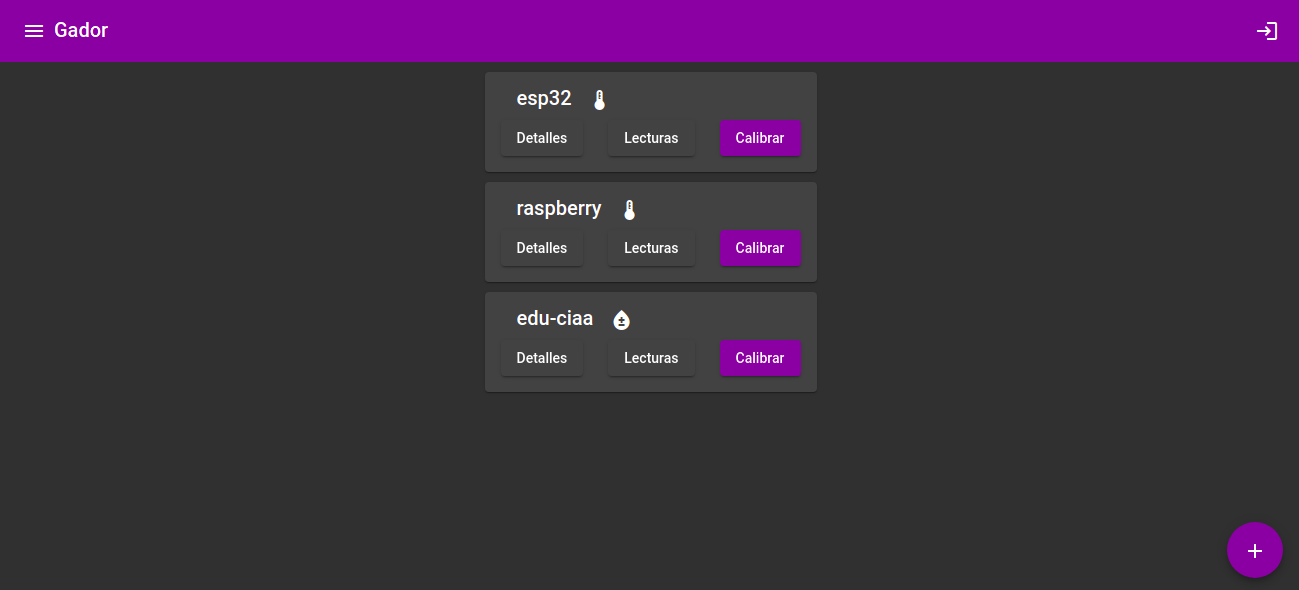
\includegraphics[width=\textwidth]{./Figures/Dispositivos.png}
	\caption{Lista de dispositivos.}
	\label{fig:ch3FrontendImg1}
\end{figure}

\begin{figure}[h]
	\centering
	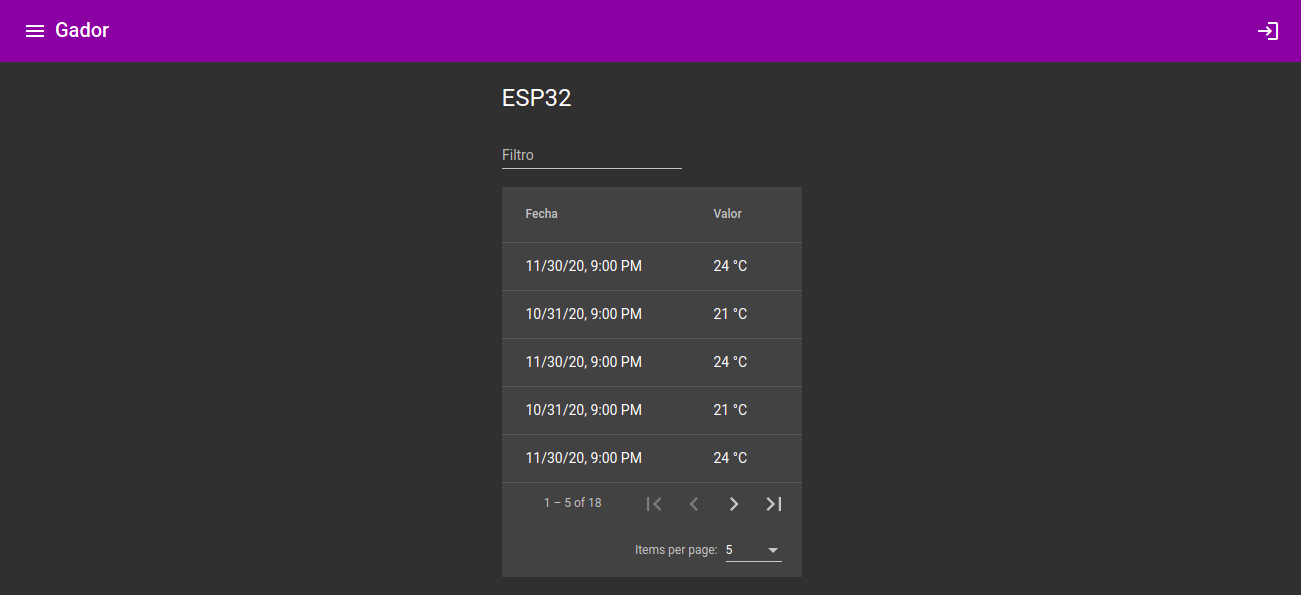
\includegraphics[width=\textwidth]{./Figures/Readings.png}
	\caption{Lecturas del sensor.}
	\label{fig:ch3FrontendImg2}
\end{figure}

\begin{figure}[h]
	\centering
	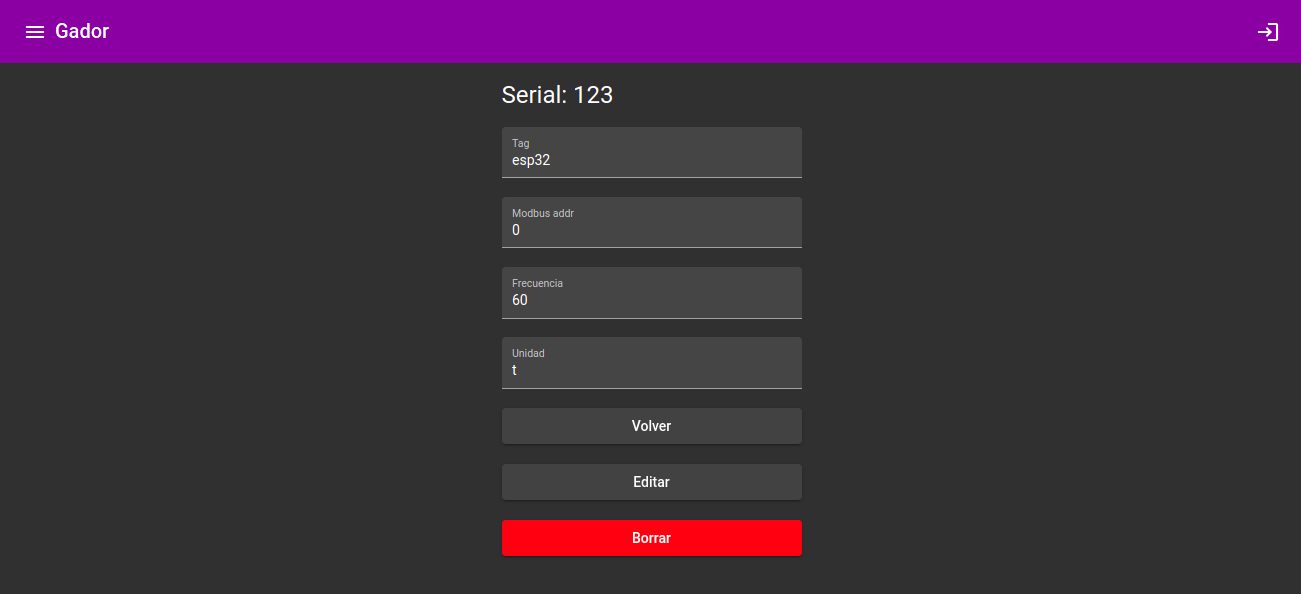
\includegraphics[width=\textwidth]{./Figures/DeviceDetails.png}
	\caption{Detalles del dispositivo.}
	\label{fig:ch3FrontendImg3}
\end{figure}
% Chapter Template

\chapter{Ensayos y Resultados} % Main chapter title

\label{Chapter4} % Change X to a consecutive number; for referencing this chapter elsewhere, use \ref{ChapterX}

%----------------------------------------------------------------------------------------
%	SECTION 1
%----------------------------------------------------------------------------------------

Párrafo introductorio del capítulo.

% Explicación de como se implementó TDD en algunos servicios y como se hicieron pruebas unitarias en otras
\section{Pruebas unitarias}

% Explicación del proceso de decición para determinar cuando debí realizar simulaciones. Descripción de las simulaciones creadas y su valides
\section{Simulaciones}

% Explicación del proceso de decición para determinar cuando debí realizar scripts. Descripción de las scripts creados y su valides
\section{Guiones y comandos}

% Recepción del cliente, sus comentarios y modificaciones realizadas para satisfacerlo
\section{Pruebas del cliente}
 
% Chapter Template

\chapter{Conclusiones} % Main chapter title

\label{Chapter5} % Change X to a consecutive number; for referencing this chapter elsewhere, use \ref{ChapterX}


%----------------------------------------------------------------------------------------

%----------------------------------------------------------------------------------------
%	SECTION 1
%----------------------------------------------------------------------------------------

Este capítulo trata sobre el valor agregado que se le dio al cliente, el aprendizaje adquirido y los siguientes pasos a seguir.

% Valor agregado al cliente y mi aprendizaje
\section{Resultados obtenidos}

El trabajo logró cumplir con los requerimientos que solicitó el cliente, y fueron listados en el capítulo \ref{Chapter1}.
Esta situación sirvió para entablar una relación positiva con el departamento de ingeniería de Gador, ya que el cliente manifestó su conformidad con los resultados obtenidos.

La planificación original del trabajo se pudo cumplir pero solo incrementado la cantidad de horas dedicadas.
El principal motivo de retraso que demandó una mayor dedicación horaria fue la poca información sobre el sistema propietario en planta.
Además, durante la cursada de la especialización se vieron temas de testeo de software que hicieron visibles ciertas fallas del trabajo.
Se dedicó un gran esfuerzo para depurar el código y lograr así una calidad de producción.

La imposibilidad de realizar pruebas dentro de la infraestructura de Gador fue un riesgo que lamentablemente se manifestó.
Solo pudo ser sorteado utilizando una máquina virtual con una licencia de uso único de seis horas de duración para verificar la comunicación.
El riesgo que por fortuna no se hizo realidad fue que alguna de las personas necesarias para realizar el trabajo se enfermara de \emph{covid-19}. O que se tomaran decisiones de prevención que afectaran la normalidad del desarrollo.

Las técnicas que mejor resultado dieron durante la creación del trabajo fue la automatización y despliegue de contenedores usando \emph{Docker} y \emph{Docker Compose} y el desarrollo orientado a pruebas.
La combinación de estos conocimientos genera software de calidad de producción que puede ser desplegado con gran facilidad en múltiples plataformas.

% Siguientes pasos para implementar el trabajo dentro del ambiente productivo de Gador
\section{Trabajo futuro}

La principal mejora a realizar es en la capa de negocios, que si bien cumple con los requerimientos del cliente, sería un salto de valor incorporar \emph{Checkmk} al sistema.
Finalmente quedaría incorporar el trabajo a la infraestructura de Gador, para lograrlo se debe crear el hardware necesario.
El siguiente paso natural es iniciar un proyecto para diseñar los sensores y puntos de agregación para tener una solución completa. 

%----------------------------------------------------------------------------------------
%	CONTENIDO DE LA MEMORIA  - APÉNDICES
%----------------------------------------------------------------------------------------

\appendix % indicativo para indicarle a LaTeX los siguientes "capítulos" son apéndices

% Incluir los apéndices de la memoria como archivos separadas desde la carpeta Appendices
% Descomentar las líneas a medida que se escriben los apéndices

%% Appendix A

\chapter{Appendix Title Here} % Main appendix title

\label{AppendixA} % For referencing this appendix elsewhere, use \ref{AppendixA}

Write your Appendix content here.
%\include{Appendices/AppendixB}
%\include{Appendices/AppendixC}

%----------------------------------------------------------------------------------------
%	BIBLIOGRAPHY
%----------------------------------------------------------------------------------------

\Urlmuskip=0mu plus 1mu\relax
\raggedright
\printbibliography[heading=bibintoc]

%----------------------------------------------------------------------------------------

\end{document}  
